\chapter{HASIL DAN PEMBAHASAN}\label{chap:bab4}
Dalam bab ini disajikan perluasan dari pemetaan $(\alpha,\beta,\gamma)$-nonekspansif pada ruang $CAT_p(0)$ yang meliputi definisi dan sifat-sifat pemetaannya. Kemudian, disajikan pula konvergensi dari skema iterasi Sabri untuk pemetaan tersebut. Selanjutnya, dilakukan simulasi numerik terkait konvergensi dari skema iterasi Sabri untuk aproksimasi titik tetap dari pemetaan $(\alpha,\beta,\gamma)$-nonekspansif. Selain itu, didapatkan pula aplikasi dari skema iterasi Sabri untuk masalah optimasi, khususnya untuk masalah minimalisasi fungsi dan rekonstruksi citra. 
\section{Pemetaan $(\alpha,\beta,\gamma)$-nonekspansif di Ruang $CAT_p(0)$}
Pada bagian ini, disajikan definisi, contoh, dan sifat-sifat dari pemetaan $(\alpha,\beta,\gamma)$-nonekspansif di ruang $CAT_p(0)$. Sifat yang didapatkan dari pemetaan ini disajikan dalam Lema \ref{Lema:dxnx*}, yang menunjukkan bahwa pemetaan ini memenuhi kondisi nonekspansif kuasi. 
Kemudian, pada Lema \ref{Lema:ineqabcnoneks} didapatkan ketaksamaan penting yang melibatkan pemetaan tersebut. Selain itu, didapatkan pula bahwa pemetaan ini memenuhi sifat \textit{demiclosedness} yang ditunjukkan oleh Lema \ref{Lema:demi}. Tiga Lema tersebut berperan penting untuk pembuktian konvergensi skema iterasi Sabri untuk aproksimasi titik tetap dari pemetaan $(\alpha,\beta,\gamma)$-nonekspansif.

Berikut ini disajikan definisi dari pemetaan $(\alpha,\beta,\gamma)$-nonekspansif di ruang $CAT_p(0)$.
\begin{defn}\label{defn:abcnoncat}
    Diberikan $(X,d,G)$ adalah ruang $CAT _p(0)$ dan $W$ adalah himpunan bagian tak kosong dari $X$, pemetaan $f:W\to W$ disebut sebagai pemetaan $(\alpha,\beta,\gamma)$-nonekspansif jika terdapat bilangan real $\alpha,\beta,\gamma\in \mathbb{R}^+\cup\{0\}$ dengan $\alpha+\gamma\leq 1,\gamma\in[0,1)$ sehingga untuk setiap $x,y\in W$ berlaku
    \begin{align}
        d(Tx,Ty)\leq \alpha d(x,y)+\beta d(x,Tx)+\gamma d(x, Ty). \label{eq:abcnoncat}
    \end{align}
\end{defn}
    Selanjutnya, diberikan contoh dari pemetaan $(\alpha,\beta,\gamma)$-nonekspansif di ruang $CAT_p(0)$. Namun, sebelum itu diberikan dulu contoh ruang yang digunakan sebagai berikut.

    Contoh berikut ini merupakan contoh dari pemetaan $(\alpha,\beta,\gamma)$-nonekspansif dengan ruang $CAT_p(0)$ yang diberikan pada Contoh \ref{con:Catp}.

    \begin{exam}\label{con:abcnon}
        Diberikan $(X,d,G)$ adalah ruang $CAT _p(0)$ sebagaimana dalam Contoh \ref{con:Catp}. Diberikan pula $W=\{(w_1,w_2,0,0,\cdots)\mid w_1\in[1,5], w_2\in[1,125]\}\subset X$. dan pemetaan $T:W\to W$ yang didefinisikan sebagai 
        \begin{align*}
            T((w_1,w_2,0,0,\cdots))=\begin{cases}
                \qty(\frac{w_1+3}{4},\frac{(w_1+3)^3}{64},0,0,\cdots), \quad &\text{jika } w_1\in [1,3)\\
                \qty(\frac{w_1+2}{4}, \frac{(w_1+2)^3}{64},0,0,\cdots), \quad &\text{jika } w_1\in [3,5].
            \end{cases}
        \end{align*}
        Pemetaan $T$ adalah pemetaan $(\frac{1}{4},\frac{1}{3},0)$-nonekspansif, tetapi bukan pemetaan nonekspansif. Titik tetap dari $T$ adalah $(1,1,0,0,\cdots)$.
    \end{exam}
        Penjelasan dari Contoh \ref{con:abcnon} diuraikan berikut ini.\\
        Diambil sebarang $u,v\in W$ dengan $u=(u_1,u_2,0,0,\cdots), ~v=(v_1,v_2,0,0,\cdots)$. Dimisalkan $D(u,v)=\alpha d(u,v)+\beta d(u,Tu)+\gamma d(u,Tv)$. 
        \begin{enumerate}[label={\textbf{Kasus \arabic*.}},align=left]
            \item Untuk $u_1,v_1\in [1,3)$, diperoleh 
            \begin{align*}
                D(u,v) =& ~\frac{1}{4}\left(|u_1-v_1|^3+|u_1^3-u_2-v_1^3+v_2|^3\right)^{\frac{1}{3}} \\
                &+ \frac{1}{3} \left(\left|u_1-\frac{u_1+3}{4}\right|^3+\bigg|u_1^3-u_2-\qty(\frac{u_1+3}{4})^3+\frac{(u_1+3)^3}{64}\bigg|^3\right)^{\frac{1}{3}}\\
                &+0\times \left(\left|u_1-\frac{v_1+3}{4}\right|^3+\bigg|u_1^3-u_2 -\qty(\frac{v_1+3}{4})^3+\frac{(v_1+3)^3}{64}\bigg|^3\right)^{\frac{1}{3}}\\
                \geq &~ \frac{1}{4}\left(|u_1-v_1|^3\right)^{\frac{1}{3}}\\
                =&~ \left|\frac{u_1+3}{4}-\frac{v_1+3}{4}\right|\\
                =&~ \Bigg(\left|\frac{u_1+3}{4}-\frac{v_1+3}{4}\right|^3           \\    &+\bigg|\qty(\frac{u_1+3}{4})^3-\frac{(u_1+3)^3}{64}-\qty(\frac{v_1+3}{4})^3+\frac{(v_1+3)^3}{64}\bigg|^3\Bigg)^{\frac{1}{3}}\\
                =& ~ d(Tu,Tv).
            \end{align*}
            \item Untuk $u_1,v_1\in [3,5]$, diperoleh 
            \begin{align*}
                D(u,v) =& ~\frac{1}{4}\left(|u_1-v_1|^3+|u_1^3-u_2-v_1^3+v_2|^3\right)^{\frac{1}{3}} \\
                &+ \frac{1}{3} \Bigg(\left|u_1-\frac{u_1+2}{4}\right|^3+\bigg|u_1^3-u_2-\qty(\frac{u_1+2}{4})^3+\frac{(u_1+2)^3}{64}\bigg|^3\Bigg)^{\frac{1}{3}}\\
                &+0\times \Bigg(\left|u_1-\frac{v_1+2}{4}\right|^3+\bigg|u_1^3-u_2 -\qty(\frac{v_1+2}{4})^3+\qty(\frac{v_1+2}{4})^3\bigg|^3\Bigg)^{\frac{1}{3}}\\
                \geq &~ \frac{1}{4}\left(|u_1-v_1|^3\right)^{\frac{1}{3}}\\
                =&~ \left|\frac{u_1+2}{4}-\frac{v_1+2}{4}\right|\\
                =&~ \Bigg(\left|\frac{u_1+2}{4}-\frac{v_1+2}{4}\right|^3           \\    &+\bigg|\qty(\frac{u_1+2}{4})^3-\frac{(u_1+2)^3}{64}-\qty(\frac{v_1+2}{4})^3+\frac{(v_1+2)^3}{64}\bigg|^3\Bigg)^{\frac{1}{3}}\\
                =& ~ d(Tu,Tv).
            \end{align*}
            \item Untuk $u_1\in [3,5]$ dan $v_1\in[1,3)$, diperoleh 
            \begin{align*}
                D(u,v) =& ~\frac{1}{4}\left(|u_1-v_1|^3+|u_1^3-u_2-v_1^3+v_2|^3\right)^{\frac{1}{3}} \\
                &+ \frac{1}{3} \Bigg(\left|u_1-\frac{u_1+2}{4}\right|^3+\bigg|u_1^3-u_2-\left(\frac{u_1+2}{4}\right)^3+\frac{(u_1+2)^3}{64}\bigg|^3\Bigg)^{\frac{1}{3}}\\
                &+0\times \Bigg(\left|u_1-\frac{v_1+3}{4}\right|^3+\bigg|u_1^3-u_2 -\qty(\frac{v_1+3}{4})^3+\frac{(v_1+3)^3}{64}\bigg|^3\Bigg)^{\frac{1}{3}}\\
                \geq &~ \frac{1}{4}\left(|u_1-v_1|^3\right)^{\frac{1}{3}}+ \frac{1}{3}\left(\qty|u_1-\frac{u_1+2}{4}|^3\right)^{\frac{1}{3}}.
            \end{align*}
            Karena $u_1\in[3,5]$, maka $\frac{1}{12}|3u_1-2|\geq \frac{7}{12}> \frac{1}{4}$, sehingga 
            \begin{align*}
                D(u,v) \geq&~ \frac{1}{4}|u_1-v_1|+\frac{1}{4}\\
                \geq&~ \qty|\frac{u_1}{4}-\frac{v_1}{4}-\frac{1}{4}|\\
                =&~ \Bigg(\qty|\frac{u_1+2}{4}-\frac{v_1+3}{4}|^3\\
                &+\qty|\qty(\frac{u_1+2}{4})^3-\frac{(u_1+2)^3}{64}-\qty(\frac{v_1+2}{4})^3+\frac{(v_1+2)^3}{64}|^3\Bigg)^{\frac{1}{3}}\\
                =&~ d(Tu,Tv).
            \end{align*}
            \item Untuk $u_1\in [1,3)$ dan $v_1\in[3,5]$, diperoleh 
            \begin{align*}
                D(u,v) =& ~\frac{1}{4}\left(|u_1-v_1|^3+|u_1^3-u_2-v_1^3+v_2|^3\right)^{\frac{1}{3}} \\
                &+ \frac{1}{3} \Bigg(\left|u_1-\frac{u_1+3}{4}\right|^3+\bigg|u_1^3-u_2-\left(\frac{u_1+3}{4}\right)^3+\frac{(u_1+3)^3}{64}\bigg|^3\Bigg)^{\frac{1}{3}}\\
                &+0\times \Bigg(\left|u_1-\frac{v_1+2}{4}\right|^3+\bigg|u_1^3-u_2 -\qty(\frac{v_1+2}{4})^3+\frac{(v_1+2)^3}{64}\bigg|^3\Bigg)^{\frac{1}{3}}\\
                \geq &~ \frac{1}{4}\left(|u_1-v_1|^3\right)^{\frac{1}{3}}+ \frac{1}{3}\left(\qty|u_1-\frac{u_1+3}{4}|^3\right)^{\frac{1}{3}} + \frac{3}{4}\left(\qty|u_1-\frac{v_1+2}{4}|^3\right)^{\frac{1}{3}}\\
                =&~ \frac{1}{4}|u_1-v_1|+\frac{1}{4}|u_1-1|.
            \end{align*}
            Diperhatikan bahwa 
            \begin{align*}
                d(Tu,Tv) =&~\Bigg(\qty|\frac{u_1+3}{4}-\frac{v_1+2}{4}|^3\\
                &+ \qty|\qty(\frac{u_1+3}{4})^3-\frac{(u_1+3)^3}{64}-\qty(\frac{v_1+2}{4})^3+\frac{(v_1+3)^3}{64}|^3\Bigg)^{\frac{1}{3}}\\
                =& ~ \frac{1}{4}|u_1-v_1+1|,
            \end{align*}
            sehingga untuk membuktikan bahwa $D(u,v)\geq d(Tu,Tv)$, akan dibuktikan bahwa 
            \begin{align*}
                f(u_1,v_1):=|u_1-v_1|+|u_1-1|-|u_1-v_1+1|\geq 0,
            \end{align*}
            untuk setiap $u_1\in [1,3)$ dan $v_1\in[3,5]$. Diamati bahwa $1\leq u_1<3\leq v_1$, sehingga 
            \begin{align*}
                f(u_1,v_1)&=v_1-u_1+u_1-1-|u_1-v_1+1|\\
                &= v_1-1-|u_1-v_1+1|.
            \end{align*}
            Jika $u_1-v_1+1< 0$, didapatkan 
            \begin{align*}
                f(u_1,v_1) = v_1-1-\qty(-(u_1-v_1+1)) = u_1\geq 1. 
            \end{align*}
            Selanjutnya, jika $u_1-v_1+1\geq 0$, diperoleh $u_1\geq v_1-1\geq 2$
            \begin{align*}
                f(u_1,v_1) = v_1-1-u_1+v_1-1 = 2v_1-u_1-2,
            \end{align*}
            sehingga 
            \begin{align*}
                \dfrac{\partial f}{\partial u_1} &= -1\neq 0 \quad \text{dan} \quad \dfrac{\partial f}{\partial v_1} = 2\neq 0.
            \end{align*}
            Hal ini berarti nilai minimumnya terdapat pada titik-titik batas. Karena $u_1\in[1,3)$ dan $u_1\geq 2$ serta $v_1\in [3,5]$, diperoleh $-3<-u_1\leq-2$ sehingga
            \begin{align*}
                f(u_1,v_1) = 2v_1-u_1-2>2v_1-5\geq 1.
            \end{align*}
                Dari uraian tersebut didapatkan bahwa $f(u_1,v_1)\geq 0$ untuk setiap $u_1\in[1,3)$ dan $v_1\in [3,5]$ sehingga berlaku pula $\alpha d(u,v)+\beta d(u,Tu)+\gamma d(u,Tv)\geq d(Tu,Tv)$.
        \end{enumerate}
        Karena semua tinjauan kasus di atas menghasilkan $\alpha d(u,v)+\beta d(u,Tu)+\gamma d(u,Tv)\geq d(Tu,Tv)$ untuk setiap $u_1,v_1\in[1,5]$, maka $T$ adalah pemetaan $(\alpha,\beta,\gamma)$-nonekspansif dengan $\alpha=\frac{1}{4},~\beta=\frac{1}{3},$ dan $\gamma=0$. Akan tetapi, $T$ bukan pemetaan nonekspansif karena untuk $u=\qty(\frac{29}{10},\frac{29^3}{1000},0,0,\dots)$ dan $v=(3,27,0,0,\dots)$, didapatkan 
            \begin{align*}
            d(Tu,Tv)=&~\Bigg(\mqty|\frac{\frac{29}{10}+3}{4}-\frac{3+2}{4}|^3\\
            &+\bigg|\bigg(\frac{\frac{29}{10}+3}{4}\bigg)^3-\frac{(\frac{29}{10}+3)^3}{64}-\frac{(3+2)^3}{64}+\bigg(\frac{3+2}{4}\bigg)^3\bigg|^3\Bigg)^{\frac{1}{3}}\\
                =&~\frac{9}{40}\\
                >&~ \frac{1}{10}\\                =&~\qty(\left|3-\frac{29}{10}\right|^3+\qty|\qty(\frac{29}{10})^3-\frac{29^3}{1000}-3^3+27|^3)^{\frac{1}{3}} \\
                =&~d(u,v).
            \end{align*}
    Selanjutnya, untuk mendapatkan titik tetap dari $T$, dicari $w=(w_1,w_2,0,0,\cdots)\in W$ sehingga $T(w)=w$. Dari definisi $T$, terdapat dua kemungkinan, yaitu
    \begin{align*}
        &\text{(i) } w_1=\frac{w_1+3}{4}, ~w_2=\frac{(w_1+3)^3}{64}, \quad \text{atau}\\
        &\text{(ii) } w_1=\frac{w_1+2}{4}, ~w_2=\frac{(w_1+2)^3}{64}.
    \end{align*}
    Dari (i) diperoleh $w_1=w_2=1\in [1,3)$, sedangkan dari (ii) diperoleh $w_1=\frac{2}{3}\notin [3,5]$. Dengan demikian, titik tetap dari $T$ adalah $(1,1,0,0,\cdots)$.
    % \begin{exam}\label{con:abcnon}
        Diberikan $(X,d,G)$ adalah ruang $CAT _p(0)$ sebagaimana dalam Contoh \ref{con:Catp}. Diberikan pula $W=\{(w_1,w_2,0,0,\cdots)\mid w_1\in[1,5], w_2\in[1,125]\}\subset X$. dan pemetaan $T:W\to W$ yang didefinisikan sebagai 
        \begin{align*}
            T((w_1,w_2,0,0,\cdots))=\begin{cases}
                \qty(\frac{w_1+3}{4},\frac{(w_1+3)^3}{64},0,0,\cdots), \quad &\text{jika } w_1\in [1,3)\\
                \qty(\frac{w_1+2}{4}, \frac{(w_1+2)^3}{64},0,0,\cdots), \quad &\text{jika } w_1\in [3,5].
            \end{cases}
        \end{align*}
        Pemetaan $T$ adalah pemetaan $(\frac{1}{4},\frac{1}{3},0)$-nonekspansif, tetapi bukan pemetaan nonekspansif. Titik tetap dari $T$ adalah $(1,1,0,0,\cdots)$.
    \end{exam}
        Penjelasan dari Contoh \ref{con:abcnon} diuraikan berikut ini.\\
        Diambil sebarang $u,v\in W$ dengan $u=(u_1,u_2,0,0,\cdots), ~v=(v_1,v_2,0,0,\cdots)$. Dimisalkan $D(u,v)=\alpha d(u,v)+\beta d(u,Tu)+\gamma d(u,Tv)$. 
        \begin{enumerate}[label={\textbf{Kasus \arabic*.}},align=left]
            \item Untuk $u_1,v_1\in [1,3)$, diperoleh 
            \begin{align*}
                D(u,v) =& ~\frac{1}{4}\left(|u_1-v_1|^3+|u_1^3-u_2-v_1^3+v_2|^3\right)^{\frac{1}{3}} \\
                &+ \frac{1}{3} \left(\left|u_1-\frac{u_1+3}{4}\right|^3+\bigg|u_1^3-u_2-\qty(\frac{u_1+3}{4})^3+\frac{(u_1+3)^3}{64}\bigg|^3\right)^{\frac{1}{3}}\\
                &+0\times \left(\left|u_1-\frac{v_1+3}{4}\right|^3+\bigg|u_1^3-u_2 -\qty(\frac{v_1+3}{4})^3+\frac{(v_1+3)^3}{64}\bigg|^3\right)^{\frac{1}{3}}\\
                \geq &~ \frac{1}{4}\left(|u_1-v_1|^3\right)^{\frac{1}{3}}\\
                =&~ \left|\frac{u_1+3}{4}-\frac{v_1+3}{4}\right|\\
                =&~ \Bigg(\left|\frac{u_1+3}{4}-\frac{v_1+3}{4}\right|^3           \\    &+\bigg|\qty(\frac{u_1+3}{4})^3-\frac{(u_1+3)^3}{64}-\qty(\frac{v_1+3}{4})^3+\frac{(v_1+3)^3}{64}\bigg|^3\Bigg)^{\frac{1}{3}}\\
                =& ~ d(Tu,Tv).
            \end{align*}
            \item Untuk $u_1,v_1\in [3,5]$, diperoleh 
            \begin{align*}
                D(u,v) =& ~\frac{1}{4}\left(|u_1-v_1|^3+|u_1^3-u_2-v_1^3+v_2|^3\right)^{\frac{1}{3}} \\
                &+ \frac{1}{3} \Bigg(\left|u_1-\frac{u_1+2}{4}\right|^3+\bigg|u_1^3-u_2-\qty(\frac{u_1+2}{4})^3+\frac{(u_1+2)^3}{64}\bigg|^3\Bigg)^{\frac{1}{3}}\\
                &+\frac{3}{4} \Bigg(\left|u_1-\frac{v_1+2}{4}\right|^3+\bigg|u_1^3-u_2 -\qty(\frac{v_1+2}{4})^3+\qty(\frac{v_1+2}{4})^3\bigg|^3\Bigg)^{\frac{1}{3}}\\
                \geq &~ \frac{1}{4}\left(|u_1-v_1|^3\right)^{\frac{1}{3}}\\
                =&~ \left|\frac{u_1+2}{4}-\frac{v_1+2}{4}\right|\\
                =&~ \Bigg(\left|\frac{u_1+2}{4}-\frac{v_1+2}{4}\right|^3           \\    &+\bigg|\qty(\frac{u_1+2}{4})^3-\frac{(u_1+2)^3}{64}-\qty(\frac{v_1+2}{4})^3+\frac{(v_1+2)^3}{64}\bigg|^3\Bigg)^{\frac{1}{3}}\\
                =& ~ d(Tu,Tv).
            \end{align*}
            \item Untuk $u_1\in [3,5]$ dan $v_1\in[1,3)$, diperoleh 
            \begin{align*}
                D(u,v) =& ~\frac{1}{4}\left(|u_1-v_1|^3+|u_1^3-u_2-v_1^3+v_2|^3\right)^{\frac{1}{3}} \\
                &+ \frac{1}{3} \Bigg(\left|u_1-\frac{u_1+2}{4}\right|^3+\bigg|u_1^3-u_2-\left(\frac{u_1+2}{4}\right)^3+\frac{(u_1+2)^3}{64}\bigg|^3\Bigg)^{\frac{1}{3}}\\
                &+\frac{3}{4} \Bigg(\left|u_1-\frac{v_1+3}{4}\right|^3+\bigg|u_1^3-u_2 -\qty(\frac{v_1+3}{4})^3+\frac{(v_1+3)^3}{64}\bigg|^3\Bigg)^{\frac{1}{3}}\\
                \geq &~ \frac{1}{4}\left(|u_1-v_1|^3\right)^{\frac{1}{3}}+ \frac{1}{3}\left(\qty|u_1-\frac{u_1+2}{4}|^3\right)^{\frac{1}{3}}.
            \end{align*}
            Karena $u_1\in[3,5]$, maka $\frac{1}{12}|3u_1-2|\geq \frac{7}{12}> \frac{1}{4}$, sehingga 
            \begin{align*}
                D(u,v) \geq&~ \frac{1}{4}|u_1-v_1|+\frac{1}{4}\\
                \geq&~ \qty|\frac{u_1}{4}-\frac{v_1}{4}-\frac{1}{4}|\\
                =&~ \Bigg(\qty|\frac{u_1+2}{4}-\frac{v_1+3}{4}|^3\\
                &+\qty|\qty(\frac{u_1+2}{4})^3-\frac{(u_1+2)^3}{64}-\qty(\frac{v_1+2}{4})^3+\frac{(v_1+2)^3}{64}|^3\Bigg)^{\frac{1}{3}}\\
                =&~ d(Tu,Tv).
            \end{align*}
            \item Untuk $u_1\in [1,3)$ dan $v_1\in[3,5]$, diperoleh 
            \begin{align*}
                D(u,v) =& ~\frac{1}{4}\left(|u_1-v_1|^3+|u_1^3-u_2-v_1^3+v_2|^3\right)^{\frac{1}{3}} \\
                &+ \frac{1}{3} \Bigg(\left|u_1-\frac{u_1+3}{4}\right|^3+\bigg|u_1^3-u_2-\left(\frac{u_1+3}{4}\right)^3+\frac{(u_1+3)^3}{64}\bigg|^3\Bigg)^{\frac{1}{3}}\\
                &+\frac{3}{4} \Bigg(\left|u_1-\frac{v_1+2}{4}\right|^3+\bigg|u_1^3-u_2 -\qty(\frac{v_1+2}{4})^3+\frac{(v_1+2)^3}{64}\bigg|^3\Bigg)^{\frac{1}{3}}\\
                \geq &~ \frac{1}{4}\left(|u_1-v_1|^3\right)^{\frac{1}{3}}+ \frac{1}{3}\left(\qty|u_1-\frac{u_1+3}{4}|^3\right)^{\frac{1}{3}} + \frac{3}{4}\left(\qty|u_1-\frac{v_1+2}{4}|^3\right)^{\frac{1}{3}}\\
                =&~ \frac{1}{4}|u_1-v_1|+\frac{1}{4}|u_1-1|+\frac{3}{16}|4u_1-v_1-2|.
            \end{align*}
            Diperhatikan bahwa 
            \begin{align*}
                d(Tu,Tv) =&~\Bigg(\qty|\frac{u_1+3}{4}-\frac{v_1+2}{4}|^3\\
                &+ \qty|\qty(\frac{u_1+3}{4})^3-\frac{(u_1+3)^3}{64}-\qty(\frac{v_1+2}{4})^3+\frac{(v_1+3)^3}{64}|^3\Bigg)^{\frac{1}{3}}\\
                =& ~ \frac{1}{4}|u_1-v_1+1|,
            \end{align*}
            sehingga untuk membuktikan bahwa $D(u,v)\geq d(Tu,Tv)$, akan dibuktikan bahwa 
            \begin{align*}
                f(u_1,v_1):=|u_1-v_1|+|u_1-1|+\frac{3}{4}|4u_1-v_1-2|-|u_1-v_1+1|\geq 0,
            \end{align*}
            untuk setiap $u_1\in [1,3)$ dan $v_1\in[3,5]$. Diamati bahwa $1\leq u_1<3\leq v_1$, sehingga 
            \begin{align*}
                f(u_1,v_1)&=v_1-u_1+u_1-1+\frac{3}{4}|4u_1-v_1-2|-|u_1-v_1+1|\\
                &= v_1-1+\frac{3}{4}|4u_1-v_1-2|-|u_1-v_1+1|.
            \end{align*}
            Dari sini, diperoleh bahwa 
            \begin{align*}
                \dfrac{\partial f}{\partial u_1} &= \frac{3(4u_1-v_1-2)}{4|4u_1-v_1-2|}\times 4-\frac{u_1-v_1+1}{|u_1-v_1+1|}\\
                &= 3\sgn{(4u_1-v_1-2)}-\sgn{(u_1-v_1+1)}\neq 0,
            \intertext{serta}
            \frac{\partial f}{\partial v_1} &= 1+\frac{3(4u_1-v_1-2)}{4|4u_1-v_1-2|}\times (-1) -\frac{u_1-v_1+1}{|u_1-v_1+1|}\times (-1) \\
            &= 1 + \frac{3}{4}\sgn{(4u_1-v_1-2)} - \sgn{(u_1-v_1+1)}\neq 0,
            \end{align*}
            artinya $f(u_1,v_1)$ tidak mempunyai titik pelana. Walaupun begitu, $f(u_1,v_1)$ mempunyai titik kritis, yaitu saat $|4u_1-v_1-2|=0$ atau $|u_1-v_1+1|=0$. Hal ini berarti nilai minimumnya berada pada titik kritis atau pada titik-titik batas domainnya. 
            \begin{enumerate}
                \item[\textbf{(a)}] \textbf{pada titik kritis}\\
                Jika $|4u_1-v_1-2|=0$, didapat $v_1=4u_1-2$ sehingga 
                \begin{align*}
                    f(u_1,v_1) = 4u_1-3-3|u_1-1|.
                \end{align*}
                Karena $u_1\geq 1$ didapat 
                \begin{align*}
                    f(u_1,v_1)=4u_1-3-3u_1+3=u_1\geq 1 >0.
                \end{align*}
                Kemudian, jika $|u_1-v_1+1|=0$, didapat $v_1=u_1+1$ sehingga
                \begin{align*}
                    f(u_1,v_1)=u_1+\frac{9}{4}|u_1-1|\geq u_1\geq 1>0.
                \end{align*}
                \item[\textbf{(b)}] \textbf{pada titik batas domain}\\
                \begin{enumerate}
                    \item Jika $u_1=1$, didapatkan 
                    \begin{align*}
                        f(u_1,v_1)\geq f(1,v_1)=v_1-1+\frac{3}{4}|2-v_1|-|2-v_1|.
                    \end{align*}
                    Karena $v_1\geq 3$, diperoleh 
                    \begin{align*}
                        f(u_1,v_1) &\geq v_1-1-\frac{1}{4}(v_1-2)= \frac{3}{4}v_1-\frac{1}{3}\geq \frac{7}{4}>0.
                    \end{align*}
                    \item Jika $u_1\to 3^{-}$, didapatkan 
                    \begin{align*}
                        f(u_1,v_1)\geq \lim_{u_1\to 3^-} f(u_1,v_1)=v_1-1+\frac{3}{4}|10-v_1|-|4-v_1|.
                    \end{align*}
                    \begin{enumerate}
                        \item Jika $v_1\in[4,5]$, diperoleh 
                        \begin{align*}
                            f(u_1,v_1)&\geq v_1-1+\frac{3}{4}(10-v_1)-(v_1-4)\\
                            &= \frac{21}{2}-\frac{3}{4}v_1 \\
                            &\geq \frac{21}{2}-\frac{15}{4}\\
                            &=\frac{27}{4}\\
                            &>0.
                        \end{align*}
                        \item Jika $v_1\in [3,4]$, didapatkan 
                        \begin{align*}
                            f(u_1,v_1)&\geq v_1-1+\frac{3}{4}(10-v_1)-(4-v_1)=\frac{5}{4}v_1+\frac{5}{2}>0.
                        \end{align*}
                    \end{enumerate}
                    \item Jika $v_1=3$, didapatkan 
                    \begin{align*}
                        f(u_1,v_1)\geq f(u_1,3) = 2+\frac{3}{4}|4u_1-5|-|u_1-2|.
                    \end{align*}
                    Karena $u_1\in [1,3)$, maka nilai maksimum dari $|u_1-2|$ adalah 1 sehingga 
                    \begin{align*}
                        f(u_1,v_1)\geq 2+\frac{3}{4}|4u_1-5|-1\geq 1>0.
                    \end{align*}
                    \item Jika $v_1=5$, didapatkan 
                    \begin{align*}
                        f(u_1,v_1)\geq f(u_1,5)=4+\frac{3}{4}|4u_1-7|-|u_1-4|.
                    \end{align*}
                    Karena $u_1\in[1,3)$, maka 
                    \begin{align*}
                        f(u_1,v_1)&\geq 4+\frac{3}{4}|4u_1-7|-(4-u_1)\\
                        &=\frac{3}{4}|4u_1-7|+u_1\\
                        &\geq u_1\\
                        &>0.
                    \end{align*}
                \end{enumerate}
                Dari uraian tersebut didapatkan bahwa $f(u_1,v_1)\geq 0$ untuk setiap $u_1\in[1,3)$ dan $v_1\in [3,5]$ sehingga berlaku pula $\alpha d(u,v)+\beta d(u,Tu)+\gamma d(u,Tv)\geq d(Tu,Tv)$.
            \end{enumerate}
        \end{enumerate}
        Karena semua tinjauan kasus di atas menghasilkan $\alpha d(u,v)+\beta d(u,Tu)+\gamma d(u,Tv)\geq d(Tu,Tv)$ untuk setiap $u_1,v_1\in[1,5]$, maka $T$ adalah pemetaan $(\alpha,\beta,\gamma)$-nonekspansif dengan $\alpha=\frac{1}{4},~\beta=\frac{1}{3},$ dan $\gamma=\frac{3}{4}$. Akan tetapi, $T$ bukan pemetaan nonekspansif karena untuk $u=\qty(\frac{29}{10},\frac{29^3}{1000},0,0,\dots)$ dan $v=(3,27,0,0,\dots)$, didapatkan 
            \begin{align*}
            d(Tu,Tv)=&~\Bigg(\mqty|\frac{\frac{29}{10}+3}{4}-\frac{3+2}{4}|^3\\
            &+\bigg|\bigg(\frac{\frac{29}{10}+3}{4}\bigg)^3-\frac{(\frac{29}{10}+3)^3}{64}-\frac{(3+2)^3}{64}+\bigg(\frac{3+2}{4}\bigg)^3\bigg|^3\Bigg)^{\frac{1}{3}}\\
                =&~\frac{9}{40}\\
                >&~ \frac{1}{10}\\                =&~\qty(\left|3-\frac{29}{10}\right|^3+\qty|\qty(\frac{29}{10})^3-\frac{29^3}{1000}-3^3+27|^3)^{\frac{1}{3}} \\
                =&~d(u,v).
            \end{align*}
    Selanjutnya, untuk mendapatkan titik tetap dari $T$, dicari $w=(w_1,w_2,0,0,\cdots)\in W$ sehingga $T(w)=w$. Dari definisi $T$, terdapat dua kemungkinan, yaitu
    \begin{align*}
        &\text{(i) } w_1=\frac{w_1+3}{4}, ~w_2=\frac{(w_1+3)^3}{64}, \quad \text{atau}\\
        &\text{(ii) } w_1=\frac{w_1+2}{4}, ~w_2=\frac{(w_1+2)^3}{64}.
    \end{align*}
    Dari (i) diperoleh $w_1=w_2=1\in [1,3)$, sedangkan dari (ii) diperoleh $w_1=\frac{2}{3}\notin [3,5]$. Dengan demikian, titik tetap dari $T$ adalah $(1,1,0,0,\cdots)$.
    
    % \begin{exam}\label{con:abcnoncat}
    %     Diberikan ruang $(\ell_3,\norm{\cdot}_3)$ dengan metrik $d(u,v)=\left(\sum_{i=1}^{+\infty} |u_i-v_i|^3\right)^{\frac{1}{3}}$. Berdasarkan Contoh \ref{con:lpcatp}, ruang tersebut adalah ruang $CAT_p(0)$. Diberikan pula $W=\{(x,y,0,0,\cdots) ~|~ y\in[1,5]\}\subset \ell_3$ dan pemetaan $T:W\to W$ yang didefinisikan sebagai 
    %     \begin{align*}
    %         T\left((x,y,0,0,\cdots)\right) = \begin{cases}
    %             (\frac{1}{3}, \frac{y+3}{4},0,0,\cdots), \qquad &\text{jika } y\in [1,3)\\
    %             (\frac{1}{3}, \frac{y+2}{4},0,0,\cdots),\qquad &\text{jika } y\in [3,5].
    %         \end{cases}
    %     \end{align*}
    %     Pemetaan $T$ adalah pemetaan $(\frac{1}{4},\frac{1}{3},\frac{3}{4})$-nonekspansif tetapi bukan pemetaan nonekspansif.

    %     Penjelasan dari contoh tersebut diberikan di bawah ini.\\
    % % \end{exam}
    % % \begin{bukti} 
    % Diambil sebarang $u,v\in W$ dengan $u=(x_1,y_1,0,0,\cdots), ~v=(x_2,y_2,0,0,\cdots)$.
    %     \begin{enumerate}[label={\textbf{Kasus \arabic*.}},align=left]
    %         \item Untuk $y_1,y_2\in [1,3)$, diperoleh 
    %         \begin{align*}
    %             \alpha d(u,v)+\beta d(u,Tu)+\gamma d(u,Tv) =& ~\frac{1}{4}\left(|x_1-x_2|^3+|y_1-y_2|^3\right)^{\frac{1}{3}} \\
    %             &+ \frac{1}{3} \left(\left|x_1-\frac{1}{3}\right|^3+\left|y_1-\frac{y_1+3}{4}\right|^3\right)^{\frac{1}{3}}\\
    %             &+\frac{3}{4} \left(\left|x_1-\frac{1}{3}\right|^3+\left|y_1-\frac{y_2+3}{4}\right|^3\right)^{\frac{1}{3}}\\
    %             \geq &~ \frac{1}{4}\left(|x_1-x_2|^3+|y_1-y_2|^3\right)^{\frac{1}{3}}\\
    %             \geq &~ \frac{1}{4}\left(|y_1-y_2|^3\right)^{\frac{1}{3}}\\
    %             =&~ \left|\frac{y_1+3}{4}-\frac{y_2+3}{4}\right|\\
    %             =&~ \left(\left|\frac{1}{3}-\frac{1}{3}\right|^3+\left|\frac{y_1+3}{4}-\frac{y_2+3}{4}\right|^3\right)^{\frac{1}{3}}\\
    %             =& ~ d(Tu,Tv).
    %         \end{align*}
    %         \item Untuk $y_1,y_2\in [3,5]$, diperoleh 
    %         \begin{align*}
    %              \alpha d(u,v)+\beta d(u,Tu)+\gamma d(u,Tv) =& ~\frac{1}{4}\left(|x_1-x_2|^3+|y_1-y_2|^3\right)^{\frac{1}{3}} \\
    %             &+ \frac{1}{3} \left(\left|x_1-\frac{1}{3}\right|^3+\left|y_1-\frac{y_1+2}{4}\right|^3\right)^{\frac{1}{3}}\\
    %             &+\frac{3}{4} \left(\left|x_1-\frac{1}{3}\right|^3+\left|y_1-\frac{y_2+2}{4}\right|^3\right)^{\frac{1}{3}}\\
    %             \geq &~ \frac{1}{4}\left(|x_1-x_2|^3+|y_1-y_2|^3\right)^{\frac{1}{3}}\\
    %             \geq &~ \frac{1}{4}\left(|y_1-y_2|^3\right)^{\frac{1}{3}}\\
    %             =&~ \left|\frac{y_1+2}{4}-\frac{y_2+2}{4}\right|\\
    %             =&~ \left(\left|\frac{1}{3}-\frac{1}{3}\right|^3+\left|\frac{y_1+2}{4}-\frac{y_2+2}{4}\right|^3\right)^{\frac{1}{3}}\\
    %             =& ~ d(Tu,Tv).
    %         \end{align*}
    %         \item Untuk $y_1\in[3,5]$ dan $y_2\in [1,3)$, diperoleh 
    %         \begin{align*}
    %             \alpha d(u,v)+\beta d(u,Tu)+\gamma d(u,Tv) =& ~\frac{1}{4}\left(|x_1-x_2|^3+|y_1-y_2|^3\right)^{\frac{1}{3}} \\
    %             &+ \frac{1}{3} \left(\left|x_1-\frac{1}{3}\right|^3+\left|y_1-\frac{y_1+2}{4}\right|^3\right)^{\frac{1}{3}}\\
    %              &+\frac{3}{4} \left(\left|x_1-\frac{1}{3}\right|^3+\left|y_1-\frac{y_2+3}{4}\right|^3\right)^{\frac{1}{3}}\\
    %              \geq &~ ~\frac{1}{4}\left(|x_1-x_2|^3+|y_1-y_2|^3\right)^{\frac{1}{3}} \\
    %              &+ \frac{1}{3} \left(\left|x_1-\frac{1}{3}\right|^3+\left|y_1-\frac{y_1+2}{4}\right|^3\right)^{\frac{1}{3}}\\
    %             \geq & ~\frac{1}{4}|y_1-y_2| + \frac{1}{3} \left|y_1-\frac{y_1+2}{4}\right|\\
    %             =&~ \frac{1}{4}|y_1-y_2| + \frac{1}{12} \left|3y_1-2\right|.
    %         \end{align*}
    %         Karena $y_1\in[3,5]$, maka $\frac{1}{12}|3y_1-2|\geq \frac{7}{12}>\frac{1}{4}$, sehingga
    %         \begin{align*}
    %             \alpha d(u,v)+\beta d(u,Tu)+\gamma d(u,Tv) \geq & ~ \frac{1}{4}|y_1-y_2| +\frac{1}{4}\\
    %             \geq&~ \left|\frac{y_1}{4}-\frac{y_2}{4}-\frac{1}{4}\right|\\
    %             \geq &~ \left(\left|\frac{1}{3}-\frac{1}{3}\right|^3+\left|\frac{y_1+2}{4}-\frac{y_2+3}{4}\right|^3\right)^\frac{1}{3}\\
    %             =&~ d(Tu,Tv).
    %         \end{align*}
    %         \item Untuk $y_1\in[1,3)$ dan $y_2\in[3,5]$, diperoleh 
    %         \begin{align*}
    %             \alpha d(u,v)+\beta d(u,Tu)+\gamma d(u,Tv) =& ~\frac{1}{4}\left(|x_1-x_2|^3+|y_1-y_2|^3\right)^{\frac{1}{3}} \\
    %             &+ \frac{1}{3} \left(\left|x_1-\frac{1}{3}\right|^3+\left|y_1-\frac{y_1+3}{4}\right|^3\right)^{\frac{1}{3}}\\
    %              &+\frac{3}{4} \left(\left|x_1-\frac{1}{3}\right|^3+\left|y_1-\frac{y_2+2}{4}\right|^3\right)^{\frac{1}{3}}\\
    %              \geq &~ \frac{1}{4}|y_1-y_2|+\frac{1}{3}\left|y_1-\frac{y_1+3}{4}\right|\\
    %              &+\frac{3}{4}\left|y_1-\frac{y_2+2}{4}\right|
    %         \end{align*}
    %         Diperhatikan bahwa 
    %         $$d(Tu,Tv)=\left(\left|\frac{1}{3}-\frac{1}{3}\right|^3+\left|\frac{y_1+3}{4}-\frac{y_2+2}{4}\right|^3\right)^\frac{1}{3} = \frac{1}{4}|y_1-y_2+1|,$$ sehingga untuk membuktikan bahwa $ \alpha d(u,v)+\beta d(u,Tu)+\gamma d(u,Tv)\geq d(Tu,Tv)$, akan dibuktikan bahwa
    %         \begin{align*}
    %             f(y_1,y_2) &=|y_1-y_2|+|y_1-1|+\frac{3}{4}\left|4y_1-y_2-2\right| - |y_1-y_2+1| \geq 0,
    %         \end{align*}
    %         untuk setiap $y_1\in[1,3)$ dan $y_2\in [3,5]$. Diamati bahwa $1\leq y_1<3\leq y_2$, sehingga 
    %         \begin{align*}
    %             f(y_1,y_2) &= y_2-y_1+y_1-1 +\frac{3}{4}|4y_1-y_2-2|-|y_1-y_2+1|\\
    %             &= y_2 -1+\frac{3}{4}|4y_1-y_2-2| - |y_1-y_2+1|.
    %         \end{align*}
    %         Dari sini, diperoleh bahwa 
    %         \begin{align*}
    %         \frac{\partial f}{\partial y_1} &= \frac{3(4y_1-y_2-2)}{4|4y_1-y_2-2|}\times 4 -\frac{y_1-y_2+1}{|y_1-y_2+1|}\\
    %         &= 3\sgn{(4y_1-y_2-2)}-\sgn{(y_1-y_2+1)} \neq 0, 
    %         \intertext{serta}
    %         \frac{\partial f}{\partial y_2} &= 1+\frac{3(4y_1-y_2-2)}{4|4y_1-y_2-2|}\times (-1) -\frac{y_1-y_2+1}{|y_1-y_2+1|}\times (-1) \\
    %         &= 1 + \frac{3}{4}\sgn{(4y_1-y_2-2)} - \sgn{(y_1-y_2+1)}\neq 0,
    %         \end{align*}
    %         artinya $f(y_1,y_2)$ tidak memiliki titik pelana. Walaupun begitu, $f(y_1,y_2)$ memiliki titik kritis, yaitu saat $|4y_1-y_2-2|=0$ atau $|y_1-y_2+1|=0$. Hal ini berarti nilai minimumnya berada pada titik kritis atau pada titik-titik batas domainnya. 
    %         \begin{enumerate}
    %             \item[\textbf{(a)}] \textbf{pada titik kritis}\\
    %             Jika $|4y_1-y_2-2|=0$, didapat $y_2=4y_1-2$ sehingga 
    %             \begin{align*}
    %                 f(y_1,y_2) = 4y_1-3-3|y_1-1|.
    %             \end{align*}
    %             Karena $y_1\geq 1$ didapat 
    %             \begin{align*}
    %                 f(y_1,y_2)=4y_1-3-3y_1+3=y_1\geq 1 >0.
    %             \end{align*}
    %             Kemudian, jika $|y_1-y_2+1|=0$, didapat $y_2=y_1+1$ sehingga
    %             \begin{align*}
    %                 f(y_1,y_2)=y_1+\frac{9}{4}|y_1-1|\geq y_1\geq 1>0.
    %             \end{align*}
    %             \item[\textbf{(b)}] \textbf{pada titik batas domain}\\
    %             \begin{enumerate}
    %                 \item Jika $y_1=1$, didapatkan 
    %                 \begin{align*}
    %                     f(y_1,y_2)\geq f(1,y_2)=y_2-1+\frac{3}{4}|2-y_2|-|2-y_2|.
    %                 \end{align*}
    %                 Karena $y_2\geq 3$, diperoleh 
    %                 \begin{align*}
    %                     f(y_1,y_2) &\geq y_2-1-\frac{1}{4}(y_2-2)= \frac{3}{4}y_2-\frac{1}{3}\geq \frac{7}{4}>0.
    %                 \end{align*}
    %                 \item Jika $y_1\to 3^{-}$, didapatkan 
    %                 \begin{align*}
    %                     f(y_1,y_2)\geq \lim_{y_1\to 3^-} f(y_1,y_2)=y_2-1+\frac{3}{4}|10-y_2|-|4-y_2|.
    %                 \end{align*}
    %                 \begin{enumerate}
    %                     \item Jika $y_2\in[4,5]$, diperoleh 
    %                     \begin{align*}
    %                         f(y_1,y_2)&\geq y_2-1+\frac{3}{4}(10-y_2)-(y_2-4)\\
    %                         &= \frac{21}{2}-\frac{3}{4}y_2 \\
    %                         &\geq \frac{21}{2}-\frac{15}{4}\\
    %                         &=\frac{27}{4}\\
    %                         &>0.
    %                     \end{align*}
    %                     \item Jika $y_2\in [3,4]$, didapatkan 
    %                     \begin{align*}
    %                         f(y_1,y_2)&\geq y_2-1+\frac{3}{4}(10-y_2)-(4-y_2)=\frac{5}{4}y_2+\frac{5}{2}>0.
    %                     \end{align*}
    %                 \end{enumerate}
    %                 \item Jika $y_2=3$, didapatkan 
    %                 \begin{align*}
    %                     f(y_1,y_2)\geq f(y_1,3) = 2+\frac{3}{4}|4y_1-5|-|y_1-2|.
    %                 \end{align*}
    %                 Karena $y_1\in [1,3)$, maka nilai maksimum dari $|y_1-2|$ adalah 1 sehingga 
    %                 \begin{align*}
    %                     f(y_1,y_2)\geq 2+\frac{3}{4}|4y_1-5|-1\geq 1>0.
    %                 \end{align*}
    %                 \item Jika $y_2=5$, didapatkan 
    %                 \begin{align*}
    %                     f(y_1,y_2)\geq f(y_1,5)=4+\frac{3}{4}|4y_1-7|-|y_1-4|.
    %                 \end{align*}
    %                 Karena $y_1\in[1,3)$, maka 
    %                 \begin{align*}
    %                     f(y_1,y_2)&\geq 4+\frac{3}{4}|4y_1-7|-(4-y_1)\\
    %                     &=\frac{3}{4}|4y_1-7|+y_1\\
    %                     &\geq y_1\\
    %                     &>0.
    %                 \end{align*}
    %             \end{enumerate}
    %             Dari uraian tersebut didapatkan bahwa $f(y_1,y_2)\geq 0$ untuk setiap $y_1\in[1,3)$ dan $y_2\in [3,5]$ sehingga berlaku pula $\alpha d(u,v)+\beta d(u,Tu)+\gamma d(u,Tv)\geq d(Tu,Tv)$.
    %         \end{enumerate}
    %     \end{enumerate}
    %     Karena semua tinjauan kasus di atas menghasilkan $\alpha d(u,v)+\beta d(u,Tu)+\gamma d(u,Tv)\geq d(Tu,Tv)$ untuk setiap $y_1,y_2\in[1,5]$, maka $T$ adalah pemetaan $(\alpha,\beta,\gamma)$-nonekspansif dengan $\alpha=\frac{1}{4},~\beta=\frac{1}{3},$ dan $\gamma=\frac{3}{4}$. Akan tetapi, $T$ bukan pemetaan nonekspansif karena untuk $u=\qty(\frac{29}{10},\frac{29^3}{1000},0,0,\dots)$ dan $v=(3,27,0,0,\dots)$, didapatkan 
    %         \begin{align*}
    %         d(Tu,Tv)=&~\Bigg(\mqty|\frac{\frac{29}{10}+3}{4}-\frac{3+2}{4}|^3\\
    %         &+\qty|\qty(\frac{\frac{29}{10}+3}{4})^3-\frac{(\frac{29}{10}+3)^3}{64}-\frac{(3+2)^3}{64}+\qty(\frac{3+2}{4})^3|^3\Bigg)^{\frac{1}{3}}\\
    %             =&~\frac{9}{40}\\
    %             >&~ \frac{1}{10}\\                =&~\qty(\left|3-\frac{29}{10}\right|^3+\qty|\qty(\frac{29}{10})^3-\frac{29^3}{1000}-3^3+27|^3)^{\frac{1}{3}} \\
    %             =&~d(u,v).
    %         \end{align*}
    % \end{exam}
    Selanjutnya, berikut ini diberikan tiga lema penting untuk pembuktian konvergensi skema iterasi Sabri. 
    \begin{lemma}\label{lemma:tutx}
    Diberikan $(X,d,G)$ adalah ruang $CAT _p(0)$ dan $W$ adalah himpunan bagian tak kosong dari $X$, serta $T:W\to W$ adalah pemetaan $(\alpha,\beta,\gamma)$-nonekspansif. Jika $u$ adalah titik tetap dari $T$, maka untuk setiap $x\in W$ berlaku $d(Tx,Tu)\leq d(x,u)$. 
    \end{lemma}
    \begin{bukti}
        Diperhatikan bahwa $u$ titik tetap dari $T$ sehingga berlaku $u=Tu$, diperoleh 
        \begin{align*}
            d(u,Tx) = d(Tu,Tx)&\leq \alpha d(u,x)+\beta d(u,Tu)+\gamma d(u,Tx)\\
            &= \alpha d(u,x) +\beta d(u,u)+ \gamma d(u,Tx)\\
            &= \alpha d(x,u) + \gamma d(u,Tx).
        \end{align*}
        Dari sini didapatkan $(1-\gamma) d(u, Tx) \leq \alpha d(x,u)$. Kemudian, karena $\alpha+\gamma\leq 1$, didapat $\alpha \leq 1-\gamma$ sehingga 
        \begin{align*}
            \frac{\alpha}{1-\gamma}\leq 1.
        \end{align*}
        Akibatnya
        \begin{align}
           d(Tx,Tu)= d(Tu,Tx)= d(u, Tx) \leq \frac{\alpha}{1-\gamma} d(x,u) \leq d(x,u).\label{ineq:titap}
        \end{align}
    \end{bukti}
    \begin{thm}
        Diberikan $(X,d,G)$ adalah ruang $CAT_p(0)$ dan $W$ adalah himpunan bagian tak kosong dari $X$, serta $T:W\to W$ adalah pemetaan $(\alpha,\beta,\gamma)$-nonekspansif. Jika $\alpha+\gamma\neq 1$ dan $T$ memiliki titik tetap, maka titik tetap dari $T$ tunggal.
    \end{thm}
    \begin{bukti}
        Misalkan $u$ dan $v$ adalah titik tetap dari $T$, maka berdasarkan Ketaksamaan \eqref{ineq:titap} diperoleh 
        \begin{align*}
            d(u,v)=d(Tu,Tv) \leq \frac{\alpha}{1-\gamma} d(u,v) 
        \end{align*} 
        Karena $\alpha,\gamma\in [0,1]$, $\gamma\neq 1$, dan $\alpha+\gamma\neq 1$, didapatkan bahwa $0\leq \frac{\alpha}{1-\gamma}<1$ sehingga $d(u,v)=0$. Dengan demikian $u=v$, yang berarti bahwa titik tetap dari $T$ tunggal. 
    \end{bukti}
    \begin{lemma}\label{Lema:ineqabcnoneks}
        Diberikan $(X,d,G)$ adalah ruang $CAT _p(0)$ dan $W$ adalah himpunan bagian tak kosong dari $X$, serta $T:W\to W$ adalah pemetaan $(\alpha,\beta,\gamma)$-nonekspansif. Untuk setiap $x,y\in W$, ketaksamaan berikut ini berlaku:
        \begin{equation}\label{eq:ineqabcnoneks}
            d(x,Ty) \leq \frac{\alpha}{1-\gamma}d(x,y)+ \frac{1+\beta}{1-\gamma}d(x,Tx).
        \end{equation}
    \end{lemma}
    \begin{bukti}
        Diamati bahwa untuk setiap $x,y\in W$ berlaku 
        \begin{align*}
            d(x,Ty) &\leq d(x,Tx)+d(Tx,Ty)\\
            &\leq d(x,Tx) + \alpha d(x,y) +\beta d(x,Tx)+\gamma d(x,Ty)\\
            &= (1+\beta)d(x,Tx) + \alpha d(x,y) + \gamma d(x,Ty). 
        \end{align*}
        Akibatnya 
        \begin{align*}
            (1-\gamma)d(x,Ty) &\leq (1+\beta)d(x,Tx) + \alpha d(x,y) \\
            \Longleftrightarrow \qquad \quad d(x,Ty)&\leq \frac{\alpha}{1-\gamma}d(x,y) + \frac{1+\beta}{1-\gamma}d(x,Tx).
        \end{align*}
    \end{bukti}
    \begin{lemma}\label{Lema:demi}
        Diberikan $(X,d,G)$ adalah ruang $CAT _p(0)$ dan $W$ adalah himpunan bagian tak kosong dari $X$. Jika $T:W\to W$ adalah pemetaan $(\alpha,\beta,\gamma)$-nonekspansif, maka $T$ memiliki sifat \textbf{demiclosedness}. 
    \end{lemma}
    \begin{bukti}
        Diambil sebarang barisan $\{x_n\}\subseteq W$ yang terbatas dan konvergen-$\Delta$ ke $u_0\in W$, serta memenuhi $\lim_{n\to\infty} d(x_n,Tx_n)=0$. Berdasarkan definisi \ref{defn:konvD}, diperoleh bahwa $u_0\in A(\{x_n\})$. Kemudian, menggunakan ketaksamaan \eqref{eq:ineqabcnoneks}, didapatkan 
        \begin{align*}
            d(x_n, Tu_0)&\leq \dfrac{\alpha}{1-\gamma}d(x_n, u_0)+\dfrac{1+\beta}{1-\gamma}d(x_n, Tx_n).
        \end{align*}
        Selanjutnya, didapatkan bahwa 
        \begin{align*}
            \limsup_{n\to \infty} d(x_n, Tu_0)\leq \limsup_{n\to \infty} \dfrac{\alpha}{1-\gamma} d(x_n, u_0) \leq \limsup_{n\to \infty} d(x_n, u_0).
        \end{align*}
        Hal ini berarti $Tu_0\in A(\{x_n\})$. Kemudian, berdasarkan Lema \ref{Lema:asimtotik}, dipunyai bahwa $A(\{x_n\})$ tepat memiliki satu elemen, yang berarti $u_0=Tu_0$. Jadi $T$ memiliki sifat \textbf{demiclosedness}. 
    \end{bukti}

\section{Konvergensi Skema Iterasi Sabri untuk Pemetaan $(\alpha,\beta,\gamma)$-nonekspansif}
Pada bagian ini disajikan skema iterasi Sabri pada ruang $CAT_p(0)$ dan hasil terkait konvergensi dari skema iterasi Sabri untuk pemetaan $(\alpha,\beta,\gamma)$-nonekspansif di ruang tersebut. Terdapat dua lema penting yang digunakan untuk membuktikan konvergensi skema tersebut, yaitu pada Lema \ref{Lema:dxnx*} yang menunjukkan bahwa barisan $d(x_{n},x^*)$ adalah barisan turun, dengan $x^*$ adalah titik tetap dari pemetaan $(\alpha,\beta,\gamma)$-nonekspansif, serta pada Lema \ref{Lema:xntxn0} yang menunjukkan bahwa barisan limit dari barisan $d(x_n,Tx_n)$ adalah 0. Kemudian, disajikan syarat eksistensi titik tetap dari pemetaan $(\alpha,\beta,\gamma)$-nonekspansif pada Teorema \ref{thm:fixtnonemp}. Hasil konvergensi dari skema ini diberikan pada Teorema \ref{thm:konvD} yang memberikan syarat cukup untuk konvergensi$-\Delta$, sedangkan syarat cukup untuk konvergensi kuat diberikan oleh Teorema \ref{thm:konvK}. 

Berikut ini diberikan skema iterasi Sabri pada ruang $CAT_p(0)$.
\begin{defn}[\textbf{Skema Iterasi Sabri}]\label{defn:sabri}
Diberikan $(X,d,G)$ adalah ruang $CAT _p(0)$ dan $W$ adalah himpunan bagian tak kosong dari $X$ yang konveks. Untuk suatu pemetaan $T:W\to W$, $x_0\in W$, dan $n\in\mathbb{N}\cup \{0\} $ didefinisikan skema iterasi Sabri pada ruang $CAT_p(0)$ sebagai berikut:
    \begin{align}\label{eq:sabricat}
       \begin{cases}
            q_n&= T\left((1-c_n)x_n \oplus c_nTx_n\right),\\
        y_n&= T(Tq_n),\\
        x_{n+1} &= T\left((1-a_n)Tq_n\oplus a_n Ty_n\right).
       \end{cases}
    \end{align}
    dengan $\{a_n\}\subseteq [0,1]$ dan $\{c_n\}\subseteq [0,1]$.
\end{defn}
Berikut ini adalah diagram alir dari skema iterasi Sabri pada ruang $CAT_p(0)$.
\begin{figure}[H]
    \centering
    \tikzstyle{startstop} = [ellipse, 
minimum width=5.5cm, 
minimum height=0.5cm,
text centered, 
draw=black]

\tikzstyle{io} = [trapezium, 
trapezium stretches=true, % A later addition
trapezium left angle=70, 
trapezium right angle=110, 
minimum width=6cm, 
minimum height=0.5cm, text centered, 
draw=black]

\tikzstyle{process} = [rectangle, 
minimum height=0.5cm, 
text centered, 
text width=8.5cm, 
draw=black]

\tikzstyle{decision} = [diamond, 
minimum width=2cm, 
minimum height=0.5cm, 
text centered, 
aspect=1.8,
inner sep=2pt,
draw=black]
\tikzstyle{arrow} = [thick,->,>=stealth]

\begin{tikzpicture}[node distance=1.4cm]

% ===== Nodes =====
\node (start) [startstop] 
{Mulai};

\node (input) [io, below of=start,align=center,yshift=-0.3cm] 
    {Inisialisasi nilai awal $x_0\in W$, $n=0$, batas galat $\varepsilon>0$, \\
    batas iterasi $N$, dan parameter iterasi $\{a_n\}_{n=1}^{\infty},\{c_n\}_{n=1}^{\infty}\subseteq (0,1)$};

\node (qn) [process, below of=input,yshift=-0.3cm] 
{$q_n = T\big((1-c_n)x_n \oplus c_n T x_n\big)$};

\node (yn) [process, below of=qn] 
{$y_n = T(Tq_n)$};

\node (xn) [process, below of=yn] 
{$x_{n+1} = T\big((1-a_n)Tq_n \oplus a_n Ty_n\big)$};

\node (decision) [decision, below of=xn, yshift=-1.4cm,align=center] 
{Apakah\\$d(x_{n+1},x^*)<\varepsilon$?\\atau $n\geq N$?};

\node (stop) [startstop, below of=decision, yshift=-1.4cm] 
{Selesai};

% ===== Arrows =====
\draw [arrow] (start) -- (input);
\draw [arrow] (input) -- (qn);
\draw [arrow] (qn) -- (yn);
\draw [arrow] (yn) -- (xn);
\draw [arrow] (xn) -- (decision);
\draw [arrow] (decision) -- node[anchor=east]{Ya} (stop);

\draw [arrow] (decision.east) -- ++(3,0) 
node[anchor=west]{Tidak}
|- (qn.east);

\end{tikzpicture}

    \caption{Diagram Alir Skema Iterasi Sabri pada Ruang $CAT_p(0)$}
    \label{fig:skemasabricat0}
\end{figure}

Untuk selanjutnya, dinotasikan $W$ sebagai himpunan bagian tak kosong yang konveks dari ruang $CAT_p(0)$ $(X,d,G)$, serta $Fix(T)$ adalah himpunan semua titik tetap dari pemetaan $T$.
\begin{lemma}\label{Lema:dxnx*}
Diberikan $T:W\to W$ adalah pemetaan $(\alpha,\beta,\gamma)$-nonekspansif dengan $Fix(T)\neq \emptyset$. Jika $\{ x_n\}$ adalah barisan yang dikonstruksi melalui skema iterasi Sabri \eqref{eq:sabricat}, maka $d(x_{n+1},x^*)\leq d(x_n,x^*)$ untuk setiap $x^*\in Fix(T)$.
\end{lemma}
\begin{bukti}
    Diambil sebarang $x^*\in Fix(T)$, berdasarkan Lema \ref{lema:d,d^p} dan \ref{lemma:tutx}, didapatkan bahwa 
    \begin{align*}
        d(q_n,x^*)&=d\left(T\qty((1-c_n)x_n\oplus c_nTx_n), Tx^*\right)\\
        &\leq d\qty((1-c_n)x_n\oplus c_nTx_n,x^*)\\
        &\leq (1-c_n)d(x_n,x^*)+c_nd(Tx_n,x^*)\\
        &\leq (1-c_n)d(x_n,x^*)+c_nd(x_n,x^*)\\
        &= d(x_n,x^*).
    \end{align*}
    Dengan cara yang sama, didapatkan pula
    \begin{align*}
        d(y_n,x^*)&=d\qty(T(Tq_n),x^*)\\
        &\leq d(Tq_n,x^*)\\
        &\leq d(q_n,x^*)\\
        &\leq d(x_n,x^*),
    \end{align*}
    serta 
    \begin{align*}
        d(x_{n+1},x^*)&= d\qty(T\qty((1-a_n)Tq_n\oplus a_n Ty_n), Tx^*)\\
        &\leq d\qty((1-a_n)Tq_n\oplus a_n Ty_n,x^*)\\
        &\leq (1-a_n)d(Tq_n,x^*)+a_n d(Ty_n,x^*)\\
        &\leq (1-a_n)d(q_n,x^*)+a_nd(y_n,x^*)\\
        &\leq (1-a_n)d(x_n,x^*)+a_n d(x_n,x^*)\\
        &= d(x_n,x^*).
    \end{align*}
\end{bukti}
\begin{lemma}\label{Lema:xntxn0}
    Diberikan $T:W\to W$ adalah pemetaan $(\alpha,\beta,\gamma)$-nonekspansif dengan $Fix(T)\neq \emptyset$. Jika $\{x_n\}$ adalah barisan yang dikonstruksi melalui skema iterasi Sabri \eqref{eq:sabricat} dengan $\{a_n\},\{c_n\}\subset (0,1)$, maka $\lim_{n\to\infty} d(x_n,Tx_n)=0$.
\end{lemma}
\begin{bukti}
    Diambil sebarang $x^*\in Fix(T)$, berdasarkan Lema \ref{lema:d,d^p} dan \ref{lemma:tutx}, didapatkan bahwa
    \begin{align*}
        \qty(d(q_n,x^*))^p &= \qty(d\qty(T\qty((1-c_n)x_n\oplus c_n Tx_n),x^*))^p\\
        &\leq \qty(d\qty((1-c_n)x_n\oplus c_nTx_n,x^*))^p\\
        &\leq (1-c_n)\qty(d(x_n,x^*))^p+c_n \qty(d(Tx_n,x^*))^p-\frac{c_n(1-c_n)}{2^{p-1}}\qty(d(x_n,Tx_n))^p.
    \end{align*}
    Karena $a\leq c_k\leq b$, diperoleh $-c_n(1-c_n)\leq a(1-b)$ sehingga 
    \begin{align*}
        \qty(d(q_n,x^*))^p&\leq (1-c_n)\qty(d(x_n,x^*))^p+c_n \qty(d(x_n,x^*))^p-\frac{a(1-b)}{2^{p-1}} \qty(d(x_n,Tx_n))^p\\
        &= \qty(d(x_n,x^*))^p-\frac{a(1-b)}{2^{p-1}}\qty(d(x_n,Tx_n))^p.
    \end{align*}
    Dengan cara yang sama, didapatkan pula
    \begin{align*}
        \qty(d(y_n,x^*))^p&=\qty(d\qty(T(Tq_n),x^*))^p\\
        &\leq \qty(d(q_n,x^*))^p\\
        &\leq \qty(d(x_n,x^*))^p-\frac{a(1-b)}{2^{p-1}}\qty(d(x_n,Tx_n))^p,
    \end{align*}
    serta
    \begin{align*}
        \qty(d(x_{n+1},x^*))^p =&~ \qty(d\qty(T\qty((1-a_n)Tq_n\oplus a_n Ty_n),x^*))^p\\
        \leq &~\qty(d\qty((1-a_n)Tq_n\oplus a_n Ty_n,x^*))^p\\
        \leq&~ (1-a_n)\qty(d(Tq_n,x^*))^p+a_n \qty(d(Ty_n,x^*))^p-\frac{c_n(1-c_n)}{2^{p-1}}\qty(d(Tq_n,Ty_n))^p\\
        \leq&~ (1-a_n)\qty(d(q_n,x^*))^p+a_n \qty(d(y_n,x^*))^p\\
        \leq&~ (1-a_n)\qty[\qty(d(x_n,x^*))^p-\frac{a(1-b)}{2^{p-1}}\qty(d(x_n,Tx_n))^p]\\
        &~+a_n \qty[\qty(d(x_n,x^*))^p-\frac{a(1-b)}{2^{p-1}}\qty(d(x_n,Tx_n))^p]\\
        =&~\qty(d(x_n,x^*))^p-\frac{a(1-b)}{2^{p-1}}\qty(d(x_n,Tx_n))^p.
    \end{align*}
    Akibatnya 
    \begin{align*}
     \qty(d(x_n,Tx_n))^p&\leq \frac{2^{p-1}}{a(1-b)}\qty[\qty(d(x_n,x^*))^p-\qty(d(x_{n+1},x^*))^p].     
    \end{align*}
    Selanjutnya, berdasarkan Lema \ref{Lema:dxnx*}, diperoleh bahwa $\{d(x_n,x^*)\}$ adalah barisan turun dan terbatas di bawah dengan batas bawah 0, sehingga $\{d(x_n,x^*)\}$ konvergen. Hal ini berarti $u_n = \qty(d(x_n,x^*))^p$ juga konvergen dan diperoleh $\lim_{n\to\infty} (u_n-u_{n+1})=0$. Akibatnya, didapatkan 
    \begin{align*}
        0\leq \lim_{n\to \infty} \qty(d(x_n,Tx_n))^p&\leq \lim_{n\to \infty} \frac{2^{p-1}}{a(1-b)}\qty[\qty(d(x_n,x^*))^p-\qty(d(x_{n+1},x^*))^p] =0.
    \end{align*}
    Jadi $\lim_{n\to\infty}d(x_n,Tx_n)=0$.
\end{bukti}


Teorema berikut ini menyajikan syarat eksistensi titik tetap dari pemetaan $(\alpha,\beta,\gamma)$-nonekspansif.
\begin{thm}\label{thm:fixtnonemp}
    Diberikan $T:W\to W$ adalah pemetaan $(\alpha,\beta,\gamma)$-nonekspansif. Jika $\{x_n\}$ adalah barisan yang dikonstruksi melalui skema iterasi Sabri \eqref{eq:sabricat} sehingga $\{x_n\}$ terbatas dan $\lim_{n\to\infty} d(x_n,Tx_n)=0$, maka $Fix(T)\neq\emptyset$.
\end{thm}
\begin{bukti}
    Diambil sebarang $x^*\in A(\{x_n\})$, maka dengan ketaksamaan \ref{eq:ineqabcnoneks}, diperoleh bahwa 
    \begin{align*}
        d(x_n,Tx^*)\leq \frac{\alpha}{1-\gamma}d(x_n,x^*)+\frac{1+\beta}{1-\gamma}d(x_n,Tx_n).
    \end{align*}
    Karena $\lim_{n\to\infty} d(x_n,Tx_n)=0$, diperoleh 
    \begin{align*}
        \limsup_{n\to\infty}d(x_n, Tx^*)=\limsup_{n\to\infty}d(x_n,x^*)\leq \limsup_{n\to\infty} d(x_n,x^*).
    \end{align*}
    Dari sini didapatkan $Tx^*\in A(\{x_n\})$, sehingga berdasarkan Lema \ref{Lema:asimtotik}, diperoleh bahwa $A(\{x_n\})$ tepat memiliki satu elemen, yang berarti $x^*=Tx^*$. Dengan demikian $Fix(T)\neq \emptyset$.
\end{bukti}
Selanjutnya, dua teorema berikut ini menyajikan hasil konvergensi dari skema Sabri, yakni konvergensi-$\Delta$ dan konvergensi kuat, untuk aproksimasi titik tetap dari pemetaan $(\alpha,\beta,\gamma)$-nonekspansif
\begin{thm}\label{thm:konvD}
    Diberikan $(X,d,G)$ adalah ruang $CAT _p(0)$ yang lengkap dan $W$ adalah himpunan bagian tak kosong dari $X$ yang tertutup dan konveks. Jika $T:W\to W$ adalah pemetaan $(\alpha,\beta,\gamma)$-nonekspansif dengan $Fix(T)\neq \emptyset$ dan $\{x_n\}$ adalah barisan yang dikonstruksi melalui skema iterasi Sabri \eqref{eq:sabricat} dengan $\{a_n\},\{c_n\}\subset (0,1)$, maka $\{x_n\}$ konvergen-$\Delta$ ke suatu titik tetap dari $T$.
\end{thm}
\begin{bukti}
    Diamati bahwa $T$ merupakan pemetaan $(\alpha,\beta,\gamma)$-nonekspansif. Dari Lema \ref{Lema:dxnx*}, didapatkan bahwa $\{d(x_n,x^*)\}$ adalah barisan turun dan terbatas di bawah dengan batas bawah 0, sehingga $\{d(x_n,x^*)\}$ konvergen untuk setiap $x^*\in Fix(T)$.
    % \begin{align}
    %     \lim_{n\to\infty} d(x_n,x^*)=0 \quad \quad \text{untuk setiap } x^*\in Fix(T).
    % \end{align}
     Kemudian, karena $Fix(T)\neq \emptyset$, maka berdasarkan Lema \ref{Lema:xntxn0}, didapatkan 
     \begin{align}
         \lim_{n\to\infty} d(x_n,Tx_n)=0.
     \end{align}
     Selanjutnya, dari Lema \ref{Lema:demi}, didapat bahwa $T$ memiliki sifat demiclosedness. Hal ini berarti semua kondisi pada Teorema \ref{thm:kondisikonvD} terpenuhi, sehingga $\{x_n\}$ konvergen$-\Delta$.
\end{bukti}
Untuk mendapatkan hasil konvergensi kuat, diperlukan syarat tambahan, yaitu himpunan $W$ haruslah merupakan himpunan kompak. 
\begin{thm}\label{thm:konvK}
     Diberikan $(X,d,G)$ adalah ruang $CAT _p(0)$ yang lengkap dan $W$ adalah himpunan bagian tak kosong dari $X$ yang tertutup, konveks, dan kompak. Jika $T:W\to W$ adalah pemetaan $(\alpha,\beta,\gamma)$-nonekspansif dengan $Fix(T)\neq \emptyset$ dan $\{x_n\}$ adalah barisan yang dikonstruksi melalui skema iterasi Sabri \eqref{eq:sabricat} dengan $\{a_n\},\{c_n\}\subset (0,1)$, maka $\{x_n\}$ konvergen kuat ke suatu titik tetap dari $T$.
\end{thm}
\begin{bukti}
    Diperhatikan bahwa $W$ adalah himpunan kompak, ini berarti ada subbarisan $\{x_{n_k}\}$ dari $\{x_n\}$ yang konvergen kuat ke $x\in W$. Akibatnya $\{x_{n_k}\}$ juga konvergen$-\Delta$ ke $x\in W$.  Dengan menggunakan fakta bahwa $W$ himpunan kompak dan $Fix(T)\neq\emptyset$, maka berdasarkan Lema \ref{Lema:xntxn0}, diperoleh
    \begin{align*}
        \lim_{k\to\infty} d(x_{n_k},Tx_{n_k})=\lim_{k\to\infty} d(x_n,Tx_n)=0.
    \end{align*}
    Kemudian dengan menggunakan sifat demiclosedness dari $T$, didapat bahwa $x\in Fix(T)$. Selanjutnya dari Lema \ref{Lema:dxnx*} didapatkan
    % \begin{align*}
    %     \lim_{k\to\infty} d(x_{n_k},x)=0.
    % \end{align*}
    % Dengan menggunakan fakta bahwa $W$ himpunan kompak, didapatkan
    \begin{align*}
        \lim_{k\to\infty} d(x_{n},x)=0.
    \end{align*}
    Dengan demikian, barisan $\{x_n\}$ konvergen kuat ke titik tetap dari $T$.
\end{bukti}

\begin{thm}
    Laju
\end{thm}
\begin{bukti}
    Diperhatikan bahwa untuk setiap $x^*\in Fix(T)$ berlaku
    \begin{align*}
        d(q_n,x^*) &= d\qty(T\qty((1-c_n)x_n\oplus c_n Tx_n),Tx^*)\\
        &\leq \frac{\alpha}{1-\gamma}d\qty((1-c_n)x_n\oplus c_n Tx_n, x^* )\\
        &\leq \frac{\alpha}{1-\gamma}\qty[(1-c_n)d(x_n,x^*)+c_n d(Tx_n,x^*)]\\
        &\leq \frac{\alpha}{1-\gamma}\qty[(1-c_n)d(x_n,x^*)+\frac{\alpha c_n}{1-\gamma}d(x_n,x^*)]\\
        &= \frac{\alpha(1-\gamma)(1-c_n)+\alpha^2 c_n}{(1-\gamma)^2}d(x_n,x^*).
    \end{align*}
    \begin{align*}
        d(y_n,x^*) &= d\qty(T(Tq_n),x^*)\\
        &\leq \frac{\alpha}{1-\gamma}d(Tq_n,x^*)\\
        &\leq \qty(\frac{\alpha}{1-\gamma})^2 d(q_n,x^*).
    \end{align*}
    \begin{align*}
        d(x_{n+1},x^*) &= d\qty(T\qty((1-a_n)Tq_n\oplus a_n Ty_n),Tx^*)\\
        &\leq \frac{\alpha}{1-\gamma}d\qty((1-a_n)Tq_n\oplus a_n Ty_n,x^*)\\
        &\leq \frac{\alpha}{1-\gamma}\qty[(1-a_n)d(Tq_n,x^*)+a_n d(Ty_n,x^*)]\\
        &\leq \qty(\frac{\alpha}{1-\gamma})^2\qty[(1-a_n)d(q_n,x^*)+a_n d(y_n,x^*)]\\
        &\leq \qty(\frac{\alpha}{1-\gamma})^2\qty[(1-a_n)d(q_n,x^*)+a_n \qty(\frac{\alpha}{1-\gamma})^2d(q_n,x^*)]\\
        &= \qty(\frac{\alpha}{1-\gamma})^2\qty[\frac{(1-a_n)(1-\gamma)^2+a_n\alpha^2}{(1-\gamma)^2}d(q_n,x^*)]\\
        &\leq \frac{\alpha^2}{(1-\gamma)^4} \qty((1-a_n)(1-\gamma)^2+a_n\alpha^2)\times \frac{\alpha(1-\gamma)(1-c_n)+\alpha^2 c_n}{(1-\gamma)^2}d(x_n,x^*)\\
        &= \frac{\alpha^3}{(1-\gamma)^6}\qty((1-a_n)(1-\gamma)^2+a_n\alpha^2)\qty((1-c_n)(1-\gamma)+c_n \alpha)d(x_n,x^*).
    \end{align*}
    Karena $\alpha\leq 1-\gamma$, didapat 
    \begin{align*}
        d(x_{n+1},x^*) &\leq \frac{\alpha^3}{(1-\gamma)^6}\qty(1-\gamma)^2\qty(1-\gamma)d(x_n,x^*) = \frac{\alpha^3}{(1-\gamma)^3}d(x_n,x^*),
    \end{align*}
    sehingga 
    \begin{align*}
        d(x_{n+1},x^*) &\leq \qty(\frac{\alpha}{1-\gamma})^3 d(x_n,x^*)\\
        &\leq  \qty(\frac{\alpha}{1-\gamma})^6 d(x_{n-1},x^*)\\
        &~~\vdots\\
        &\leq  \qty(\frac{\alpha}{1-\gamma})^{3(n+1)} d(x_0,x^*).
    \end{align*}
    Jika terdapat $\alpha+\gamma\neq 1$, didapatkan $\lim_{n\to\infty} d(x_n,x^*)=0$.
\end{bukti}
\begin{bukti}
    \begin{align*}
        d(q_n,x^*) &=d\qty(T\qty((1-c_n)x_n\oplus c_n Tx_n),Tx^*)\\
        &\leq bd\qty((1-c_n)x_n\oplus c_n Tx_n, x^* )\\
        &\leq bm\qty[(1-c_n)d(x_n,x^*)+c_n d(Tx_n,x^*)]\\
        &\leq bm\qty[(1-c_n)d(x_n,x^*)+bc_nd(x_n,x^*)]\\
        &= bm\qty(1-c_n(1-b))d(x_n,x^*).
    \end{align*}
    \begin{align*}
        d(y_n,x^*) &= d\qty(T(Tq_n),x^*)\\
        &\leq bd(Tq_n,x^*)\\
        &\leq b^2 d(q_n,x^*).
    \end{align*}
    \begin{align*}
        d(x_{n+1},x^*) &= d\qty(T\qty((1-a_n)Tq_n\oplus a_n Ty_n),Tx^*)\\
        &\leq bd\qty((1-a_n)Tq_n\oplus a_n Ty_n,x^*)\\
        &\leq bm\qty[(1-a_n)d(Tq_n,x^*)+a_n d(Ty_n,x^*)]\\
        &\leq b^2m\qty[(1-a_n)d(q_n,x^*)+a_n d(y_n,x^*)]\\
        &\leq b^2m\qty[(1-a_n)d(q_n,x^*)+a_n b^2d(q_n,x^*)]\\
        &= b^2m\qty[(1-a_n(1-b^2))d(q_n,x^*)]\\
        &\leq b^2m (1-a_n(1-b^2))(bm(1-c_n(1-b)))d(x_n,x^*)\\
        &= b^3m^2 (1-a_n(1-b^2))(1-c_n(1-b))d(x_n,x^*).
    \end{align*}
\end{bukti}

\section{Percobaan Numerik}
Pada bagian ini, dilakukan percobaan numerik untuk menguji laju konvergensi dari skema iterasi Sabri dibanding dengan skema iterasi lainnya. Untuk percobaan ini, terlebih dahulu dikenalkan skema iterasi JK yang dikembangkan pada ruang $CAT_p(0)$ oleh Salisu sebagai berikut. 
\begin{defn}[\textbf{Skema Iterasi JK}]\cite{Salisu2022}\label{defn:jk}
% Diberikan $(X,d,G)$ adalah ruang $CAT _p(0)$ dan $W$ adalah himpunan bagian tak kosong dari $X$ yang konveks. 
Untuk suatu pemetaan $T:W\to W$, $x_0\in W$, dan $n\in\mathbb{N}\cup \{0\} $ didefinisikan skema iterasi JK pada ruang $CAT_p(0)$ sebagai berikut:
    \begin{align}\label{eq:jkcat}
       \begin{cases}
            q_n &= (1-c_n)x_n \oplus c_nTx_n,\\
        y_n&= Tq_n,\\
        x_{n+1} &= T\left((1-a_n)Tq_n\oplus a_n Ty_n\right),
       \end{cases}
    \end{align}
    dengan $\{a_n\}\subseteq [0,1]$ dan $\{c_n\}\subseteq [0,1]$.
\end{defn}
Selain itu, berikut ini dikenalkan pula skema iterasi Thakur, Abbas, dan Agarwal pada ruang $CAT_p(0)$. 
\begin{defn}[\textbf{Skema Iterasi Thakur}]\label{defn:thakur}
% Diberikan $(X,d,G)$ adalah ruang $CAT _p(0)$ dan $W$ adalah himpunan bagian tak kosong dari $X$ yang konveks. 
Untuk suatu pemetaan $T:W\to W$, $x_0\in W$, dan $n\in\mathbb{N}\cup \{0\} $ didefinisikan skema iterasi Thakur pada ruang $CAT_p(0)$ sebagai berikut:
    \begin{align}\label{eq:thakurcat}
       \begin{cases}
            q_n&= (1-c_n)x_n \oplus c_nTx_n,\\
        y_n&= T((1-a_n)x_n\oplus a_nq_n),\\
        x_{n+1} &= Ty_n,
       \end{cases}
    \end{align}
    dengan $\{a_n\}\subseteq [0,1]$ dan $\{c_n\}\subseteq [0,1]$.
\end{defn}
\begin{defn}[\textbf{Skema Iterasi Abbas}]\label{defn:abbas}
% Diberikan $(X,d,G)$ adalah ruang $CAT _p(0)$ dan $W$ adalah himpunan bagian tak kosong dari $X$ yang konveks. 
Untuk suatu pemetaan $T:W\to W$, $x_0\in W$, dan $n\in\mathbb{N}\cup \{0\} $ didefinisikan skema iterasi Abbas pada ruang $CAT_p(0)$ sebagai berikut:
    \begin{align}\label{eq:abbascat}
       \begin{cases}
            q_n&= (1-c_n)x_n \oplus c_nTx_n,\\
        y_n&= (1-b_n)Tx_n\oplus b_nTq_n,\\
        x_{n+1} &= (1-a_n)Ty_n\oplus a_n Tq_n,
       \end{cases}
    \end{align}
    dengan $\{a_n\}\subseteq [0,1]$, $\{b_n\}\subseteq [0,1]$, dan $\{c_n\}\subseteq [0,1]$.
\end{defn}
\begin{defn}[\textbf{Skema Iterasi Agarwal}]\label{defn:agarwal}
% Diberikan $(X,d,G)$ adalah ruang $CAT _p(0)$ dan $W$ adalah himpunan bagian tak kosong dari $X$ yang konveks. 
Untuk suatu pemetaan $T:W\to W$, $x_0\in W$, dan $n\in\mathbb{N}\cup \{0\} $ didefinisikan skema iterasi Agarwal pada ruang $CAT_p(0)$ sebagai berikut:
    \begin{align}\label{eq:agarwalcat}
       \begin{cases}
        y_n&= (1-c_n)x_n\oplus a_n Tx_n,\\
        x_{n+1} &= (1-a_n)Tx_n\oplus a_n Ty_n,
       \end{cases}
    \end{align}
    dengan $\{a_n\}\subseteq [0,1]$ dan $\{c_n\}\subseteq [0,1]$.
\end{defn}

Percobaan numerik dilakukan dengan perangkat lunak Google Colab yang menggunakan bahasa pemrograman Python. Digunakan beberapa variasi parameter, baik dari nilai awal $x_0$ maupun parameter di skema iterasinya, yaitu barisan $\{a_n\},\{b_n\},\{c_n\}$.
Pemetaan dan ruang yang digunakan dalam percobaan ini diambil dari Contoh \ref{con:abcnon} yang memiliki titik tetap $x^*=(1,1,0,0,\dots)$. 

Untuk hasil numerik tiap iterasi, digunakan batas galat $d(x_{n+1},x_n)<10^{-6}$, sedangkan untuk jumlah iterasi yang diperlukan untuk konvergen dari masing-masing skema iterasi, digunakan batas galat $d(x_{n+1},x_n)<10^{-16}$. Dalam percobaan ini, laju konvergensi skema iterasi Sabri \eqref{eq:sabricat} dibandingkan dengan Skema iterasi JK \eqref{eq:jkcat}, Thakur \eqref{eq:thakurcat}, Abbas \ref{eq:abbascat}, dan Agarwal \eqref{eq:agarwalcat}. Kode dari percobaan ini dapat dilihat pada Lampiran A.1.

Pada \ref{tab:sabjk}, \ref{tab:sabthkur}, \ref{tab:sababb}, dan \ref{tab:sabag} disajikan hasil numerik dari tiap iterasi dengan nilai awal $(2,3,0,0,\dots)$ dan parameter $a_n=0.92, b_n=0.83, c_n=0.81$ untuk setiap $n\in\mathbb{N}$ hingga batas galat $d(x_{n+1},x_n)<10^{-6}$.

\begin{table}[H]
    \centering
    \caption{Hasil numerik skema iterasi Sabri dan JK}
    \begin{tabular}{ccc}
\hline
\textbf{Iterasi} & \multicolumn{2}{c}{\textbf{Nilai $x_n$ hingga $d(x_{n+1},x_n)<10^{-6}$}} \\
\hline
\textbf{n} & \textbf{Sabri} & \textbf{JK} \\
\hline
0 & (2.000000, 3.000000, 0, 0, \dots) & (2.000000, 3.000000, 0, 0, \dots) \\
1 & (1.000843, 1.002532, 0, 0, \dots) & (1.007605, 1.022988, 0, 0, \dots) \\
2 & (1.000001, 1.000002, 0, 0, \dots) & (1.000058, 1.000174, 0, 0, \dots) \\
3 & (1.000000, 1.000000, 0, 0, \dots) & (1.000000, 1.000001, 0, 0, \dots) \\
4 & (1, 1, 0, 0, \dots) & (1.000000, 1.000000, 0, 0, \dots) \\
\hline
\end{tabular}
    \label{tab:sabjk}
\end{table}

\begin{table}[H]
    \centering
        \caption{Hasil numerik skema iterasi Sabri dan Thakur}
    \begin{tabular}{ccc}
\hline
\textbf{Iterasi} & \multicolumn{2}{c}{\textbf{Nilai $x_n$ hingga $d(x_{n+1},x_n)<10^{-6}$}} \\
\hline
\textbf{n} & \textbf{Sabri} & \textbf{Thakur} \\
\hline
0 & (2.000000, 3.000000, 0, 0, \dots) & (2.000000, 3.000000, 0, 0, \dots) \\
1 & (1.000843, 1.002532, 0, 0, \dots) & (1.027569, 1.085007, 0, 0, \dots) \\
2 & (1.000001, 1.000002, 0, 0, \dots) & (1.000760, 1.002282, 0, 0, \dots) \\
3 & (1.000000, 1.000000, 0, 0, \dots) & (1.000021, 1.000063, 0, 0, \dots) \\
4 & (1, 1, 0, 0, \dots) & (1.000001, 1.000002, 0, 0, \dots) \\
5 & (1, 1, 0, 0, \dots) & (1.000000, 1.000000, 0, 0, \dots) \\
\hline
\end{tabular}
    \label{tab:sabthkur}
\end{table}

\begin{table}[H]
    \centering
        \caption{Hasil numerik skema iterasi Sabri dan Abbas}
    \begin{tabular}{ccc}
\hline
\textbf{Iterasi} & \multicolumn{2}{c}{\textbf{Nilai $x_n$ hingga $d(x_{n+1},x_n)<10^{-6}$}} \\
\hline
\textbf{n} & \textbf{Sabri} & \textbf{Abbas} \\
\hline
0 & (2.000000, 3.000000, 0, 0, \dots) & (2.000000, 3.000000, 0, 0, \dots) \\
1 & (1.000843, 1.002532, 0, 0, \dots) & (1.092754, 1.304869, 0, 0, \dots) \\
2 & (1.000001, 1.000002, 0, 0, \dots) & (1.008603, 1.026033, 0, 0, \dots) \\
3 & (1.000000, 1.000000, 0, 0, \dots) & (1.000798, 1.002396, 0, 0, \dots) \\
4 & (1, 1, 0, 0, \dots) & (1.000074, 1.000222, 0, 0, \dots) \\
5 & (1, 1, 0, 0, \dots) & (1.000007, 1.000021, 0, 0, \dots) \\
6 & (1, 1, 0, 0, \dots) & (1.000001, 1.000002, 0, 0, \dots) \\
7 & (1, 1, 0, 0, \dots) & (1.000000, 1.000000, 0, 0, \dots) \\
\hline
\end{tabular}
    \label{tab:sababb}
\end{table}

% \begin{longtable}{ccc}
% \caption{\centering Hasil numerik skema iterasi Sabri dan Abbas}\\
% \hline
% \textbf{Iterasi} & \multicolumn{2}{c}{\textbf{Nilai $x_n$ hingga $d(x_{n+1},x_n)<10^{-6}$}} \\
% \hline
% \textbf{n} & \textbf{Sabri} & \textbf{Abbas} \\
% \hline
% \endfirsthead 
% \multicolumn{3}{c}{ \thetable{} -- Lanjutan dari halaman sebelumnya} \\
% \hline
% \textbf{n} & \textbf{Sabri} & \textbf{Abbas} \\
% \hline
% \endhead 
% \hline
% 0 & (2.000000, 3.000000, 0, 0, \dots) & (2.000000, 3.000000, 0, 0, \dots) \\
% 1 & (1.007270, 1.021970, 0, 0, \dots) & (1.109842, 1.367048, 0, 0, \dots) \\
% 2 & (1.000053, 1.000159, 0, 0, \dots) & (1.012065, 1.036634, 0, 0, \dots) \\
% 3 & (1.000000, 1.000001, 0, 0, \dots) & (1.001325, 1.003981, 0, 0, \dots) \\
% 4 & (1, 1, 0, 0, \dots) & (1.000146, 1.000437, 0, 0, \dots) \\
% 5 & (1, 1, 0, 0, \dots) & (1.000016, 1.000048, 0, 0, \dots) \\
% 6 & (1, 1, 0, 0, \dots) & (1.000002, 1.000005, 0, 0, \dots) \\
% 7 & (1, 1, 0, 0, \dots) & (1.000000, 1.000001, 0, 0, \dots) \\
% \hline
% \label{tab:sababb}
% \end{longtable}


\begin{table}[H]
    \centering
        \caption{Hasil numerik skema iterasi Sabri dan Agarwal}
    \begin{tabular}{ccc}
\hline
\textbf{Iterasi} & \multicolumn{2}{c}{\textbf{Nilai $x_n$ hingga $d(x_{n+1},x_n)<10^{-6}$}} \\
\hline
\textbf{n} & \textbf{Sabri} & \textbf{Agarwal} \\
\hline
0 & (2.000000, 3.000000, 0, 0, \dots) & (2.000000, 3.000000, 0, 0, \dots) \\
1 & (1.000843, 1.002532, 0, 0, \dots) & (1.110275, 1.368648, 0, 0, \dots) \\
2 & (1.000001, 1.000002, 0, 0, \dots) & (1.012161, 1.036927, 0, 0, \dots) \\
3 & (1.000000, 1.000000, 0, 0, \dots) & (1.001341, 1.004028, 0, 0, \dots) \\
4 & (1, 1, 0, 0, \dots) & (1.000148, 1.000444, 0, 0, \dots) \\
5 & (1, 1, 0, 0, \dots) & (1.000016, 1.000049, 0, 0, \dots) \\
6 & (1, 1, 0, 0, \dots) & (1.000002, 1.000005, 0, 0, \dots) \\
7 & (1, 1, 0, 0, \dots) & (1.000000, 1.000001, 0, 0, \dots) \\
8 & (1, 1, 0, 0, \dots) & (1.000000, 1.000000, 0, 0, \dots) \\
\hline
\end{tabular}
    \label{tab:sabag}
\end{table}

\begin{longtable}{cccccc}
\caption{\centering Galat $d(x_n, x^*)$}\label{tab:galat}\\
\hline
% \textbf{Iterasi} & \multicolumn{5}{c}{\textbf{Nilai Galat $d(x_n, x^*)$}} \\
% \hline
$\mathbf{n}$ & \textbf{Sabri} & \textbf{JK} & \textbf{Thakur} & \textbf{Abbas} & \textbf{Agarwal} \\
\hline
\endfirsthead 
\multicolumn{6}{c}{ \thetable{} -- Lanjutan dari halaman sebelumnya} \\
\hline
$\mathbf{n}$ & \textbf{Sabri} & \textbf{JK} & \textbf{Thakur} & \textbf{Abbas} & \textbf{Agarwal} \\
\hline
\endhead 
\hline
% \multicolumn{3}{|c|}{{Lanjut pada halaman berikutnya}} \\
\endfoot 
\hline
\endlastfoot
\hline
1 & $5.0\times10^{0}$ & $5.0\times10^{0}$ & $5.0\times10^{0}$ & $5.0\times10^{0}$ & $5.0\times10^{0}$ \\
2 & $8.4\times10^{-4}$ & $7.5\times10^{-3}$ & $2.6\times10^{-2}$ & $8.4\times10^{-2}$ & $9.8\times10^{-2}$ \\
3 & $7.1\times10^{-7}$ & $5.7\times10^{-5}$ & $7.3\times10^{-4}$ & $7.8\times10^{-3}$ & $1.0\times10^{-2}$ \\
4 & $5.9\times10^{-10}$ & $4.3\times10^{-7}$ & $2.0\times10^{-5}$ & $7.2\times10^{-4}$ & $1.1\times10^{-3}$ \\
5 & $5.0\times10^{-13}$ & $3.3\times10^{-9}$ & $5.6\times10^{-7}$ & $6.7\times10^{-5}$ & $1.3\times10^{-4}$ \\
6 & $4.4\times10^{-16}$ & $2.5\times10^{-11}$ & $1.5\times10^{-8}$ & $6.2\times10^{-6}$ & $1.4\times10^{-5}$ \\
7 & 0 & $1.9\times10^{-13}$ & $4.2\times10^{-10}$ & $5.7\times10^{-7}$ & $1.5\times10^{-6}$ \\
8 & 0 & $1.5\times10^{-15}$ & $1.1\times10^{-11}$ & $5.3\times10^{-8}$ & $1.7\times10^{-7}$ \\
9 & 0 & 0 & $3.2\times10^{-13}$ & $4.9\times10^{-9}$ & $1.9\times10^{-8}$ \\
10 & 0 & 0 & $9.1\times10^{-15}$ & $4.6\times10^{-10}$ & $2.1\times10^{-9}$ \\
11 & 0 & 0 & $2.2\times10^{-16}$ & $4.2\times10^{-11}$ & $2.3\times10^{-10}$ \\
12 & 0 & 0 & 0 & $3.9\times10^{-12}$ & $2.6\times10^{-11}$ \\
13 & 0 & 0 & 0 & $3.6\times10^{-13}$ & $2.8\times10^{-12}$ \\
14 & 0 & 0 & 0 & $3.4\times10^{-14}$ & $3.1\times10^{-13}$ \\
15 & 0 & 0 & 0 & $2.8\times10^{-15}$ & $3.5\times10^{-14}$ \\
16 & 0 & 0 & 0 & $4.4\times10^{-16}$ & $3.7\times10^{-15}$ \\
17 & 0 & 0 & 0 & 0 & $4.4\times10^{-16}$ \\
\hline
\end{longtable}
% \begin{table}[H]
%     \centering
%         \caption{Galat $d(x_n, x^*)$}
%     \label{tab:galat}
%     \begin{tabular}{cccccc}
%     \hline
%     $\mathbf{n}$ & \textbf{Sabri} & \textbf{JK} & \textbf{Thakur} & \textbf{Abbas} & \textbf{Agarwal} \\
%     \hline
%     1 & 0.007270 & 0.032859 & 0.056397 & 0.109842 & 0.225588 \\
%     2& 0.000053 & 0.001080 & 0.003181 & 0.012065 & 0.050890 \\
% 3 & 0.000000 & 0.000035 & 0.000179 & 0.001325 & 0.011480 \\
% 4 & NaN & 0.000001 & 0.000010 & 0.000146 & 0.002590 \\
% 5 & NaN & 0.000000 & 0.000001 & 0.000016 & 0.000584 \\
% 6 & NaN & NaN & NaN & 0.000002 & 0.000132 \\
% 7 & NaN & NaN & NaN & 0.000000 & 0.000030 \\
% 8 & NaN & NaN & NaN & NaN & 0.000007 \\
% 9 & NaN & NaN & NaN & NaN & 0.000002 \\
% 10 & NaN & NaN & NaN & NaN & 0.000000 \\
% \hline
%     \end{tabular}
% \end{table}
\begin{figure}[H]
    \centering
    \includegraphics[width=\linewidth]{Bab_4/galatpercobaan.png}
    \caption{Galat $d(x_{n+1},x_n)$ (dalam log) vs iterasi}
    \label{fig:galatperc}
\end{figure}
Dengan galat kurang dari $10^{-6}$, skema iterasi Sabri hanya membutuhkan 3 iterasi dibanding dengan JK (4 iterasi), Thakur (5 iterasi), Abbas (7 iterasi), dan Agarwal (8 iterasi). Pada \ref{tab:galat}, diberikan pula nilai galat $d(x_n,x^*)$ dari tiap iterasi. \ref{fig:galatperc} juga memberikan gambaran mengenai penurunan galatnya. 


Selanjutnya, pada \ref{tab:paramkonstan}, \ref{tab:paramturun}, \ref{tab:paramnaik}, \ref{tab:paramnaikturun}, dan \ref{tab:paramturunnaik}, disajikan jumlah iterasi yang diperlukan sampai batas galat $d(x_{n+1},x^*)<10^{-16}$ dari masing-masing skema iterasi dengan nilai awal dan parameter yang berbeda. Nilai awal dipilih secara acak dengan batasan nilainya berada pada domain pemetaan yang digunakan. Pada tabel-tabel tersebut parameter barisan $\{a_n\}$ dan $\{c_n\}$ berturut-turut dipilih dengan kondisi konstan-konstan, turun-turun, naik-naik, naik-turun, dan turun-naik. 
% \begin{longtable}{cccccc}
% \caption{\centering Iterasi dengan parameter $a_n = 0.42, b_n=0.83, c_n=0.31$}\\
% \hline
% $\mathbf{n}$ & \textbf{Sabri} & \textbf{JK} & \textbf{Thakur} & \textbf{Abbas} & \textbf{Agarwal} \\
% \hline
% \endfirsthead 
% \multicolumn{6}{c}{ \thetable{} -- Lanjutan dari halaman sebelumnya} \\
% \hline
% $\mathbf{n}$ & \textbf{Sabri} & \textbf{JK} & \textbf{Thakur} & \textbf{Abbas} & \textbf{Agarwal} \\
% \hline
% \endhead 
% \hline
% (2.0, 3.0, 0, 0, \dots) & 9 & 12 & 14 & 18 & 26 \\
% (3.0, 4.0, 0, 0, \dots) & 9 & 12 & 14 & 19 & 26 \\
% (4.0, 1.0, 0, 0, \dots) & 9 & 12 & 14 & 19 & 26 \\
% (1.5, 4.0, 0, 0, \dots) & 9 & 12 & 14 & 18 & 26 \\
% (2.7, 4.2, 0, 0, \dots) & 9 & 12 & 14 & 19 & 26 \\
% (5.0, 1.8, 0, 0, \dots) & 9 & 12 & 15 & 19 & 27 \\
% (3.1, 3.5, 0, 0, \dots) & 9 & 12 & 14 & 19 & 26 \\
% \hline
% \label{tab:paramkonstan}
% \end{longtable}
\begin{table}[H]
\caption{Iterasi dengan parameter $a_n = 0.92, b_n=0.83, c_n=0.81$}
    \centering
    \begin{tabular}{cccccc}
\hline
\textbf{Nilai Awal} & \multicolumn{5}{c}{\textbf{Jumlah Iterasi}} \\
\hline
$x_0$ & Sabri & JK & Thakur & Abbas & Agarwal \\
\hline
(2.0, 3.0, 0, 0, \dots) & 8 & 10 & 13 & 18 & 19 \\
(3.0, 4.0, 0, 0, \dots) & 8 & 10 & 13 & 18 & 19 \\
(4.0, 1.0, 0, 0, \dots) & 8 & 10 & 13 & 18 & 19 \\
(1.5, 4.0, 0, 0, \dots) & 8 & 10 & 12 & 18 & 19 \\
(2.7, 4.2, 0, 0, \dots) & 8 & 10 & 13 & 18 & 19 \\
(5.0, 1.8, 0, 0, \dots) & 8 & 10 & 13 & 19 & 20 \\
(3.1, 3.5, 0, 0, \dots) & 8 & 10 & 13 & 18 & 19 \\
\hline
\end{tabular}
    \label{tab:paramkonstan}
\end{table}
\begin{table}[H]
\caption{Iterasi dengan parameter $a_n =\frac{n^2}{n^3+1}, b_n=\frac{2}{n+3},c_n=\frac{4n+2}{{7n+4}}.$}
    \centering
    \begin{tabular}{cccccc}
\hline
\textbf{Nilai Awal} & \multicolumn{5}{c}{\textbf{Jumlah Iterasi}} \\
\hline
$x_0$ & Sabri & JK & Thakur & Abbas & Agarwal \\
\hline
(2.0, 3.0, 0, 0, \dots) & 10 & 13 & 15 & 16 & 28 \\
(3.0, 4.0, 0, 0, \dots) & 10 & 13 & 15 & 16 & 28 \\
(4.0, 1.0, 0, 0, \dots) & 10 & 13 & 16 & 17 & 28 \\
(1.5, 4.0, 0, 0, \dots) & 10 & 13 & 15 & 16 & 27 \\
(2.7, 4.2, 0, 0, \dots) & 10 & 13 & 15 & 17 & 28 \\
(5.0, 1.8, 0, 0, \dots) & 10 & 13 & 16 & 17 & 29 \\
(3.1, 3.5, 0, 0, \dots) & 10 & 13 & 15 & 16 & 28 \\
\hline
\end{tabular}
    \label{tab:paramturun}
\end{table}
\begin{table}[H]
\caption{Iterasi dengan parameter $a_n =1- \frac{\sqrt{4n+9}}{2n+13}, b_n=0.8,c_n=1-\frac{n^2}{\sqrt{n^7+3}}.$}
    \centering
    \begin{tabular}{cccccc}
\hline
\textbf{Nilai Awal} & \multicolumn{5}{c}{\textbf{Jumlah Iterasi}} \\
\hline
$x_0$ & Sabri & JK & Thakur & Abbas & Agarwal \\
\hline
(2.0, 3.0, 0, 0, \dots) & 8 & 10 & 13 & 16 & 19 \\
(3.0, 4.0, 0, 0, \dots) & 8 & 10 & 13 & 16 & 19 \\
(4.0, 1.0, 0, 0, \dots) & 8 & 11 & 13 & 16 & 19 \\
(1.5, 4.0, 0, 0, \dots) & 8 & 10 & 13 & 16 & 19 \\
(2.7, 4.2, 0, 0, \dots) & 8 & 11 & 13 & 16 & 19 \\
(5.0, 1.8, 0, 0, \dots) & 8 & 11 & 13 & 17 & 20 \\
(3.1, 3.5, 0, 0, \dots) & 8 & 10 & 13 & 16 & 19 \\
\hline
\end{tabular}
    \label{tab:paramnaik}
\end{table}
\begin{table}[H]
\caption{Iterasi dengan parameter $a_n = 1-\frac{n^3}{n^5+1}, b_n=\frac{1}{n+1},c_n=\frac{3n+4}{5n^2+4}.$}
    \centering
    \begin{tabular}{cccccc}
\hline
\textbf{Nilai Awal} & \multicolumn{5}{c}{\textbf{Jumlah Iterasi}} \\
\hline
$x_0$ & Sabri & JK & Thakur & Abbas & Agarwal \\
\hline
(2.0, 3.0, 0, 0, \dots) & 8 & 11 & 15 & 25 & 27 \\
(3.0, 4.0, 0, 0, \dots) & 8 & 11 & 15 & 25 & 27 \\
(4.0, 1.0, 0, 0, \dots) & 8 & 11 & 15 & 26 & 27 \\
(1.5, 4.0, 0, 0, \dots) & 8 & 11 & 14 & 25 & 26 \\
(2.7, 4.2, 0, 0, \dots) & 8 & 11 & 15 & 26 & 27 \\
(5.0, 1.8, 0, 0, \dots) & 8 & 11 & 15 & 26 & 27 \\
(3.1, 3.5, 0, 0, \dots) & 8 & 11 & 15 & 26 & 27 \\
\hline
\end{tabular}
    \label{tab:paramnaikturun}
\end{table}
\begin{table}[H]
\caption{Iterasi dengan parameter $a_n = \frac{n^5+1}{5n^7+9}, b_n=1-\frac{3}{n+5},c_n=1-\frac{\sqrt{n^3+8}}{5n^5+9}.$}
    \centering
    \begin{tabular}{cccccc}
\hline
\textbf{Nilai Awal} & \multicolumn{5}{c}{\textbf{Jumlah Iterasi}} \\
\hline
$x_0$ & Sabri & JK & Thakur & Abbas & Agarwal \\
\hline
(2.0, 3.0, 0, 0, \dots) & 9 & 11 & 16 & 13 & 29 \\
(3.0, 4.0, 0, 0, \dots) & 9 & 12 & 16 & 13 & 29 \\
(4.0, 1.0, 0, 0, \dots) & 9 & 12 & 16 & 14 & 29 \\
(1.5, 4.0, 0, 0, \dots) & 9 & 11 & 15 & 13 & 28 \\
(2.7, 4.2, 0, 0, \dots) & 9 & 12 & 16 & 13 & 29 \\
(5.0, 1.8, 0, 0, \dots) & 9 & 12 & 16 & 14 & 29 \\
(3.1, 3.5, 0, 0, \dots) & 9 & 12 & 16 & 13 & 29 \\
\hline
\end{tabular}
    \label{tab:paramturunnaik}
\end{table}
Hasil tersebut menunjukkan bahwa skema iterasi Sabri memiliki laju konvergensi yang lebih baik daripada yang lainnya secara numerik. Dengan parameter tertentu, skema tersebut hanya membutuhkan 8 iterasi untuk konvergen ke titik tetapnya dengan galat kurang dari $10^{-16}$. Secara analitik, skema iterasi Sabri lebih cepat karena nilai galat asimtotiknya, yaitu $\lambda\leq \frac{\alpha^3}{(1-\gamma)^3}$, sedangkan untuk JK dan Thakur adalah $\lambda\leq \frac{\alpha^2}{(1-\gamma)^2}$ yang ditunjukkan dalam teorema berikut ini. 
\begin{thm}
Diberikan $(X,d,G)$ adalah ruang $CAT _p(0)$ yang lengkap dan $W$ adalah himpunan bagian tak kosong dari $X$ yang tertutup, konveks, dan kompak. Jika $T:W\to W$ adalah pemetaan $(\alpha,\beta,\gamma)$-nonekspansif dengan $\alpha+\gamma<1$, $Fix(T)\neq \emptyset$, serta $\{x_n\}$ adalah barisan yang dikonstruksi melalui skema iterasi JK \eqref{eq:jkcat} dengan $\{a_n\},\{c_n\}\subset (0,1)$, maka $\{x_n\}$ memiliki laju konvergensi linear dengan galat asimtotik $\lambda\leq \frac{\alpha^2}{(1-\gamma)^2}$.
\end{thm}
\begin{bukti}
    Berdasarkan Lema \ref{lema:d,d^p} dan Lema \ref{lemma:tutx}, diperoleh bahwa untuk setiap $x^*\in Fix(T)$ berlaku
    \begin{align*}
        d(q_n,x^*) &= d\qty((1-c_n)x_n\oplus c_n Tx_n,Tx^*)\\
        &\leq (1-c_n)d(x_n,x^*)+c_n d(Tx_n,x^*)\\
        &\leq (1-c_n)d(x_n,x^*)+\frac{\alpha c_n}{1-\gamma}d(x_n,x^*)\\
        &= \frac{(1-\gamma)(1-c_n)+\alpha c_n}{(1-\gamma)}d(x_n,x^*),\\
        d(y_n,x^*) &= d\qty(Tq_n,x^*)\\
        &\leq \frac{\alpha}{1-\gamma}d(q_n,x^*),\\
        d(x_{n+1},x^*) &= d\qty(T\qty((1-a_n)Tq_n\oplus a_n Ty_n),Tx^*)\\
        &\leq \frac{\alpha}{1-\gamma}d\qty((1-a_n)Tq_n\oplus a_n Ty_n,x^*)\\
        &\leq \frac{\alpha}{1-\gamma}\qty[(1-a_n)d(Tq_n,x^*)+a_n d(Ty_n,x^*)]\\
        &\leq \qty(\frac{\alpha}{1-\gamma})^2\qty[(1-a_n)d(q_n,x^*)+a_n d(y_n,x^*)]\\
        &\leq \qty(\frac{\alpha}{1-\gamma})^2\qty[(1-a_n)d(q_n,x^*)+a_n \frac{\alpha}{1-\gamma}d(q_n,x^*)]\\
        &= \qty(\frac{\alpha}{1-\gamma})^2\qty[\frac{(1-a_n)(1-\gamma)+a_n\alpha}{(1-\gamma)}d(q_n,x^*)]\\
        &\leq \frac{\alpha^2}{(1-\gamma)^3} \qty((1-a_n)(1-\gamma)+a_n\alpha)\times \frac{(1-\gamma)(1-c_n)+\alpha c_n}{(1-\gamma)}d(x_n,x^*)\\
        &= \frac{\alpha^2}{(1-\gamma)^4}\qty((1-a_n)(1-\gamma)+a_n\alpha)\qty((1-c_n)(1-\gamma)+c_n \alpha)d(x_n,x^*).
    \end{align*}
    Karena $\alpha< 1-\gamma$, didapat 
    \begin{align}
        d(x_{n+1},x^*) &\leq \frac{\alpha^2}{(1-\gamma)^4}\qty(1-\gamma)\qty(1-\gamma)d(x_n,x^*) = \frac{\alpha^2}{(1-\gamma)^2}d(x_n,x^*),
    \end{align}
    sehingga 
    \begin{align*}
        \lim_{n\to\infty} \dfrac{d(x_{n+1},x^*)}{d(x_n,x^*)} \leq \frac{\alpha^2}{(1-\gamma)^2}<+\infty
    \end{align*}
    Hal ini berarti $\{x_n\}$ memiliki laju konvergensi linear dengan galat asimtotik $\lambda\leq \frac{\alpha^2}{(1-\gamma)^2}$.
\end{bukti}
\begin{thm}
Diberikan $(X,d,G)$ adalah ruang $CAT _p(0)$ yang lengkap dan $W$ adalah himpunan bagian tak kosong dari $X$ yang tertutup, konveks, dan kompak. Jika $T:W\to W$ adalah pemetaan $(\alpha,\beta,\gamma)$-nonekspansif dengan $\alpha+\gamma<1$, $Fix(T)\neq \emptyset$, serta $\{x_n\}$ adalah barisan yang dikonstruksi melalui skema iterasi Thakur \eqref{eq:thakurcat} dengan $\{a_n\},\{c_n\}\subset (0,1)$, maka $\{x_n\}$ memiliki laju konvergensi linear dengan galat asimtotik $\lambda\leq \frac{\alpha^2}{(1-\gamma)^2}$.
\end{thm}
\begin{bukti}
    Berdasarkan Lema \ref{lema:d,d^p} dan Lema \ref{lemma:tutx}, diperoleh bahwa untuk setiap $x^*\in Fix(T)$ berlaku
    \begin{align*}
        d(q_n,x^*) &= d\qty((1-c_n)x_n\oplus c_n Tx_n,Tx^*)\\
        &\leq (1-c_n)d(x_n,x^*)+c_n d(Tx_n,x^*)\\
        &\leq (1-c_n)d(x_n,x^*)+\frac{\alpha c_n}{1-\gamma}d(x_n,x^*)\\
        &= \frac{(1-\gamma)(1-c_n)+\alpha c_n}{(1-\gamma)}d(x_n,x^*),\\
        d(y_n,x^*) &= d\qty(T\qty((1-a_n)x_n\oplus a_nq_n),x^*)\\
        &\leq \frac{\alpha}{1-\gamma}d\qty((1-a_n)x_n\oplus a_n q_n,x^*)\\
        &\leq \frac{\alpha}{1-\gamma} \qty[(1-a_n)d(x_n,x^*)+a_n d(q_n,x^*)],\\
        d(x_{n+1},x^*) &= d(Ty_n,Tx^*)\\
        &\leq \frac{\alpha}{(1-\gamma)}d(y_n,x^*)\\
        &\leq \frac{\alpha^2}{(1-\gamma)^2} \qty[(1-a_n)d(x_n,x^*)+a_n d(q_n,x^*)]\\
        &\leq \frac{\alpha^2}{(1-\gamma)^2} \qty[(1-a_n)d(x_n,x^*)+a_n \frac{(1-\gamma)(1-c_n)+\alpha c_n}{(1-\gamma)}d(x_n,x^*)]
    \end{align*}
    Karena $\alpha< 1-\gamma$, didapat 
    \begin{align}
        d(x_{n+1},x^*) &\leq \frac{\alpha^2}{(1-\gamma)^2}d(x_n,x^*),
    \end{align}
    sehingga 
    \begin{align*}
        \lim_{n\to\infty} \dfrac{d(x_{n+1},x^*)}{d(x_n,x^*)} \leq \frac{\alpha^2}{(1-\gamma)^2}<+\infty
    \end{align*}
    Hal ini berarti $\{x_n\}$ memiliki laju konvergensi linear dengan galat asimtotik $\lambda\leq \frac{\alpha^2}{(1-\gamma)^2}$.
\end{bukti}
% Hasil ini secara intuitif dapat dijelaskan dari struktur iterasi Sabri yang melibatkan komposisi pemetaan nonekspansif $T$ secara berlapis pada setiap langkah iterasi, sehingga jarak barisan iterasi terhadap titik tetap berkurang lebih signifikan pada setiap iterasi dibandingkan dengan skema iterasi lainnya.

\section{Aplikasi pada Masalah Optimasi}
Dalam bagian ini disajikan bahwa skema iterasi Sabri dapat digunakan pada masalah optimasi, khususnya untuk masalah minimalisasi dan rekonstruksi citra. 
\subsection{Masalah Minimalisasi}
Diberikan suatu himpunan tak kosong $X$ dan $f:X\to\mathbb{R}\cup\{\infty\}$ adalah suatu pemetaan. Masalah pencarian titik yang meminimumkan fungsi $f$ dapat diformulasikan sebagai mencari nilai 
\begin{align}\label{eq:minprob}
    x\in X \quad \text{sehingga}\quad f(x)\leq f(y), \quad \text{untuk setiap}\quad y\in X.
\end{align}
Permasalahan ini merupakan permasalahan penting dalam bidang optimasi dan analisis tak linier. Selanjutnya, diperkenalkan operator resolvent dari suatu fungsi.
\begin{defn}
    Diberikan $(X,d,G)$ adalah ruang $CAT _p(0)$ dan $f:X\to \mathbb{R}\cup\{+\infty\}$ adalah suatu fungsi. Untuk $\lambda>0$, operator resolvent $\lambda$ dari $f$ didefinisikan sebagai
    \begin{align}
        J^f_{\lambda}(x) = \text{argmin}_{y\in X} \qty[f(y)+\frac{1}{2\lambda}\qty(d(x,y))^2].
    \end{align}
\end{defn}
\begin{exam}
    Diberikan $(\mathbb{R}^2,\|\cdot\|_2)$ adalah ruang Banach yang juga merupakan $CAT_p(0)$. Misalkan $f:\mathbb{R}^2\to \mathbb{R}\cup\{+\infty\}$ adalah fungsi yang didefinisikan sebagai $f(x_1,x_2) = |x_1| + |x_2|$ untuk setiap $(x_1,x_2)\in \mathbb{R}^2$. Untuk $\lambda>0$ dan $x=(x_1,x_2)\in \mathbb{R}^2$, operator resolvent $J^f_{\lambda}$ dari $f$ adalah sebagai berikut.
    \begin{align*}
        J^f_{\lambda}(x) &= \text{argmin}_{y\in \mathbb{R}^2} \qty[|y_1| + |y_2| + \frac{1}{2\lambda}\qty(\norm{(x_1,y_2)-(y_1,y_2)}_2)^2]\\
        &= \text{argmin}_{y\in \mathbb{R}^2} \qty[|y_1| + |y_2| + \frac{1}{2\lambda}\qty((x_1 - y_1)^2 + (x_2 - y_2)^2)].
    \end{align*}
    % Dengan memisahkan variabel $y_1$ dan $y_2$, diperoleh
    % \begin{align*}  
    %     J^f_{\lambda}(x) &= \left(\text{argmin}_{y_1\in \mathbb{R}} \qty[|y_1| + \frac{1}{2\lambda}(x_1 - y_1)^2], \text{argmin}_{y_2\in \mathbb{R}} \qty[|y_2| + \frac{1}{2\lambda}(x_2 - y_2)^2]\right)\\
    %     &= \left(sgn(x_1)\max\qty(|x_1| - \lambda, 0), sgn(x_2)\max\qty(|x_2| - \lambda, 0)\right).
    % \end{align*}
\end{exam}

Untuk fungsi yang memenuhi kondisi konveks dan \textit{proper lower semi-continuous}, himpunan solusi dari masalah \eqref{eq:minprob} sama dengan himpunan titik tetap dari operator resolvent $J^f_{\lambda}$ (lihat proposisi 6.5 pada \cite{ArizaRuiz2014}). Berikut ini diberikan definisi dari fungsi yang memenuhi kondisi tersebut dengan contoh yang diberikan pada Contoh \ref{con:fkonvk}.

\begin{defn}\cite{Khamsi2017}\label{def:konvgeodesik}
    Diberikan $(X,d,G)$ adalah ruang $CAT _p(0)$. Suatu fungsi $f:X\to \mathbb{R}\cup \{+\infty\}$ disebut konveks secara geodesik jika untuk setiap $t\in(0,1)$ dan $x,y\in X$, berlaku
    \begin{align*}
        f(tx\oplus (1-t)y)\leq tf(x)+(1-t)f(y).
    \end{align*}
\end{defn}
\begin{defn}\cite{Salisu2022}
    Diberikan $(X,d,G)$ adalah ruang $CAT _p(0)$. Suatu fungsi $f:X\to \mathbb{R}\cup \{+\infty\}$ disebut \textit{proper} jika himpunan $D(f):=\{x\in X\mid f(x)<+\infty\}\neq \emptyset$.
\end{defn}
\begin{defn}\cite{Salisu2022}
    Diberikan $(X,d,G)$ adalah ruang $CAT _p(0)$. Suatu fungsi $f:X\to \mathbb{R}\cup \{+\infty\}$ disebut \textit{lower semi-continuous} pada suatu titik $x\in D(f)$ jika $f(x)\leq \liminf_{n\to\infty} f(x_n)$ untuk setiap barisan $\{x_n\}_{n=1}^{\infty}$ yang konvergen di $D(f)$ dengan limit $x\in X$. Jika $f$ \textit{lower semi-continuous} pada setiap titik di $D(f)$, maka $f$ disebut \textit{lower semi-continuous} pada $X$.
\end{defn}

Berdasarkan hal tersebut, didapatkan Teorema berikut. 
\begin{thm}\label{thm:apl1}
    Diberikan $(X,d,G)$ adalah ruang $CAT _p(0)$ dan $f:X\to\mathbb{R}\cup\{+\infty\}$ adalah fungsi yang memenuhi kondisi konveks dan \textit{proper lower semi-continuous}. Untuk $x\in X$, barisan $\{x_n\}_{n=1}^{\infty}$ yang didefinisikan sebagai 
    \begin{align}
        \begin{cases}
            q_n &= J^f_{\lambda}\qty((1-c_n)x_n\oplus c_n J^f_{\lambda} (x_n))\\
            y_n &= J^f_{\lambda} \qty(J^f_{\lambda} (q_n))\\
            x_{n+1} &=J^f_{\lambda} \qty((1-a_n)J^f_{\lambda} (q_n)\oplus a_n J^f_{\lambda} (y_n)),
        \end{cases}
    \end{align}
    dengan $\{a_n\}_{n=1}^{\infty},\{c_n\}_{n=1}^{\infty}\subseteq [a,b]\subset (0,1)$ konvergen-$\Delta$ ke solusi dari permasalahan \eqref{eq:minprob}. Jika $X$ kompak, maka $\{x_n\}_{n=1}^{\infty}$ konvergen kuat. 
\end{thm}
\begin{bukti}
    Dengan menggunakan Lema 4 di \cite{Jost1995}, diketahui bahwa $J^f_{\lambda}$ merupakan pemetaan nonekspansif, sehingga merupakan pemetaan $(\alpha,\beta,\gamma)$-nonekspansif juga. Akibatnya, dengan Teorema \ref{thm:konvD} diperoleh bahwa $\{x_n\}_{n=1}^{\infty}$ konvergen-$\Delta$ ke titik tetap dari $J^f_{\lambda}$. Jika $X$ kompak, Teorema \ref{thm:konvK}, menjamin bahwa konvergensinya kuat. Karena titik tetap dari $J^f_{\lambda}$ sama dengan solusi dari permasalahan \eqref{eq:minprob}, artinya Teorema \ref{thm:apl1} terbukti. 
\end{bukti}

Sebagai gambaran, dilakukan simulasi untuk contoh berikut ini. 
\begin{exam}\label{con:fkonvk}
    Diberikan $(X,d,G)$ adalah ruang $CAT _p(0)$ sebagaimana Contoh \ref{con:Catp} dan $W=\{(x_1,x_2,0,0,\dots)\mid x_1,x_2\in X\}$. Suatu fungsi $f:W\to \mathbb{R}\cup\{+\infty\}$ yang didefinisikan sebagai 
    \begin{align}
        f\qty(x) = 20\qty|x_2-x_1^3|^3+|26-x_1|^3, \quad \text{untuk}\quad x=(x_1,x_2,0,0,\dots)\in W,
    \end{align}
    merupakan fungsi tak konveks pada definisi klasiknya, tetapi konveks secara geodesik dengan geodesik sebagaimana pada Contoh \ref{con:Catp}. Lebih lanjut, $f$ merupakan fungsi yang \textit{proper lower semicontinuous} dan mencapai nilai minimum saat $x_1=26$ dan $x_2=26^3$. 
\end{exam}
Penjelasan dari Contoh \ref{con:fkonvk} diberikan sebagai berikut. 
\begin{enumerate}
    \item Pertama, ditunjukkan bahwa $f$ tak konveks dalam definisi klasiknya, yaitu $f$ memenuhi ketaksamaan
    \begin{align*}
        f\qty((1-t)w + tz) \leq (1-t)f(w) + t f(z),
    \end{align*}
    untuk setiap $t\in(0,1)$ dan $w,z\in W$. Untuk menunjukkan bahwa $f$ tidak konveks dalam definisi klasik, digunakan matriks Hessian, yaitu 
    
    \begin{align*}
        H = \begin{bmatrix}
           \dfrac{\partial^2 f}{\partial x_1^2} & \dfrac{\partial^2 f}{\partial x_1x_2} \vspace*{0.3cm}\\ 
           \dfrac{\partial^2 f}{\partial x_2x_1} & \dfrac{\partial^2 f}{\partial x_2^2}
        \end{bmatrix}.
    \end{align*}
    Ingat kembali bahwa suatu fungsi $f:W\to \mathbb{R}$ adalah konveks jika dan hanya jika matriks Hessian $H$ adalah matriks semidefinit positif untuk setiap $x\in W$ (lihat \cite{Boyd2004}).
    Dapat dihitung bahwa 
    \begin{align*}
        \dfrac{\partial f}{\partial x_1} &= -180(x_2x_1^2-x_1^5)|x_2-x_1^3|-3(26-x_1)|26-x_1|.\\
        \dfrac{\partial^2 f}{\partial x_1^2} &= -180\qty((2x_1x_2-5x_1^4)|x_2-x_1^3|-\frac{3x_1^4(x_2-x_1^3)^2}{|x_2-x_1^3|}) + \frac{6(26-x_1)^2}{|26-x_1|}.\\
        \dfrac{\partial^2 f}{\partial x_1x_2} &= \frac{-360x_1^2(x_2-x_1^3)^2}{|x_2-x_1^3|}.\\
        \dfrac{\partial f}{\partial x_2} &= 60(x_2-x_1^3)|x_2-x_1|^3.\\
        \dfrac{\partial^2 f}{\partial x_2 x_1} &= \frac{-360x_1^2(x_2-x_1^3)^2}{|x_2-x_1^3|}.\\
        \dfrac{\partial^2 f}{\partial x_2^2} &= 60\qty(|x_2-x_1^3|+\frac{(x_2-x_1^3)^2}{|x_2-x_1^3|}).
    \end{align*}
    Jika diambil $x_1=1$ dan $x_2=5$, diperoleh 
    \begin{align*}
        H = \begin{bmatrix}
            -1290 & -1440\\
            -1440 & 480
        \end{bmatrix}.
    \end{align*}
    Diperhatikan bahwa $H$ mempunyai persamaan karakteristik $p(\lambda)=\lambda^2+810\lambda-2692800$ dengan akar-akar 
    \begin{align*}
        \lambda_{1,2} = \frac{-810 \pm \sqrt{810^2-4(2692800)}}{2},
    \end{align*}
    yang jelas mempunyai akar negatif. Jadi ada $x\in W$ sehingga matriks Hessian $H$ mempunyai nilai eigen negatif, yang berarti $H$ bukan matriks semidefinit positif. Akibatnya $f$ bukanlah fungsi konveks dalam definisi klasik. 
    \item Kedua, ditunjukkan bahwa $f$ memenuhi Definisi \ref{def:konvgeodesik}, yaitu fungsi konveks secara geodesik. Sebelum itu, diperhatikan bahwa fungsi $p(x)=|x|^3$ adalah fungsi konveks, karena $p''(x)=\frac{6x^2}{|x|}\geq 0$ untuk setiap $x\in \mathbb{R}\backslash \{0\}$. Dengan fakta tersebut, didapatkan bahwa untuk setiap $t\in(0,1)$ dan $w,z\in X$ berlaku
    \begin{align*}
        f\qty((1-t)w\oplus tz) =~& f\big((1-t)w_1+tz_1, \qty((1-t)w_1+tz_1)^3\\
        &\quad\,\,    -(1-t)(w_1^3-w_2)-t(z_1^3-z_2)\big)\\
        =~& 20\qty|(1-t)(w_2-w_1^3)+t(z_2-z_1)^3|^3\\
        ~&+\qty|26-\qty((1-t)w_1+tz_1)|^3\\
        \leq ~& 20 \qty((1-t)|w_2-w_1^3|^3+t|z_2-z_1^3|^3)\\
        ~&+ \qty |(1-t)(26-w_1)+t(26-z_1)|^3\\
        \leq ~& (1-t) \qty(20|w_2-w_1^3|^3+|26-w_1|^3)\\
        ~&+ t\qty(20|z_2-z_1^3|^3+|26-z_1|^3)\\
        =~& (1-t)f(w)+tf(z).
    \end{align*}
    Jadi $f$ adalah fungsi konveks secara geodesik. 
\end{enumerate}
Selanjutnya, diperhatikan bahwa $(0,0,0,\dots)\in D(f)$ sehingga $D(f)=\{x\in X\mid f(x)<+\infty\}\neq\emptyset$, yang berarti $f$ adalah fungsi \textit{proper}. Diperhatikan pula bahwa $f$ adalah fungsi kontinu, yang berarti juga memenuhi kondisi \textit{lower semicontinuous}. Dalam hal ini kondisi pada Teorema \ref{thm:konvK} terpenuhi. Diperhatikan bahwa 
nilai minimum dari fungsi $f$ pada Contoh \ref{con:fkonvk} adalah $0$, yang dicapai saat $x_2-x_1^3=0$ dan $26-x_1=0$, atau pada titik $x^*=(26, 17576, 0,0,\dots)$. Dengan demikian, berdasarkan Teorema \ref{thm:apl1}, barisan yang dihasilkan dari skema iterasi Sabri dan JK konvergen ke titik $x^*$. 

Untuk ilustrasi, dilakukan simulasi numerik untuk Contoh \ref{con:fkonvk} dengan perangkat lunak Google Colab yang menggunakan bahasa pemrograman python. Kode dari program ini dapat dilihat pada Lampiran A.2. Pada simulasi ini digunakan parameter $\lambda=20$, $a_n=0.74$, dan $c_n=0.93$, serta nilai awal $x_0=(10, 15, 0, 0, \dots)$. Simulasi dilakukan sebanyak 72 iterasi yang hasilnya dapat dilihat pada \ref{tab:simulasimin} dan \ref{tab:errsimulasi}. Galat dari simulasi ini juga digambarkan sebagai grafik dengan koordinat-$y$ berskala log yang disajikan pada \ref{fig:galatsim}.
\begin{longtable}{|c|c|c|}
\caption{\centering Hasil simulasi sebanyak 72 iterasi untuk Contoh \ref{con:fkonvk} dengan skema iterasi Sabri dan JK}\label{tab:simulasimin}\\
\hline
\textbf{n} & \textbf{Sabri} & \textbf{JK} \\
\hline
\endfirsthead 
\multicolumn{3}{c}{ \thetable{} -- Lanjutan dari halaman sebelumnya} \\
\hline
\textbf{n} & \textbf{Sabri} & \textbf{JK} \\
\hline
\endhead 
\hline
% \multicolumn{3}{|c|}{{Lanjut pada halaman berikutnya}} \\
\endfoot 
\hline
\endlastfoot
\hline
0 & (10.00000, 15.00000, 0, 0, \dots) & (10.00000, 15.00000, 0, 0, \dots) \\
1 & (25.77581, 17125.21877, 0, 0, \dots) & (23.07560, 12287.24784, 0, 0, \dots) \\
2 & (25.99383, 17563.49526, 0, 0, \dots) & (25.97620, 17527.77515, 0, 0, \dots) \\
3 & (25.99765, 17571.24240, 0, 0, \dots) & (25.99458, 17565.01472, 0, 0, \dots) \\
4 & (25.99860, 17573.17051, 0, 0, \dots) & (25.99726, 17570.44169, 0, 0, \dots) \\
5 & (25.99902, 17574.00765, 0, 0, \dots) & (25.99821, 17572.37307, 0, 0, \dots) \\
6 & (25.99925, 17574.46912, 0, 0, \dots) & (25.99868, 17573.33297, 0, 0, \dots) \\
7 & (25.99939, 17574.75968, 0, 0, \dots) & (25.99896, 17573.90002, 0, 0, \dots) \\
8 & (25.99949, 17574.95880, 0, 0, \dots) & (25.99915, 17574.27215, 0, 0, \dots) \\
9 & (25.99956, 17575.10350, 0, 0, \dots) & (25.99928, 17574.53424, 0, 0, \dots) \\
10 & (25.99961, 17575.21329, 0, 0, \dots) & (25.99937, 17574.72839, 0, 0, \dots) \\
11 & (25.99965, 17575.29936, 0, 0, \dots) & (25.99945, 17574.87778, 0, 0, \dots) \\
12 & (25.99969, 17575.36861, 0, 0, \dots) & (25.99951, 17574.99618, 0, 0, \dots) \\
13 & (25.99972, 17575.42551, 0, 0, \dots) & (25.99955, 17575.09225, 0, 0, \dots) \\
14 & (25.99974, 17575.47307, 0, 0, \dots) & (25.99959, 17575.17173, 0, 0, \dots) \\
15 & (25.99976, 17575.51342, 0, 0, \dots) & (25.99962, 17575.23855, 0, 0, \dots) \\
16 & (25.99978, 17575.54807, 0, 0, \dots) & (25.99965, 17575.29549, 0, 0, \dots) \\
17 & (25.99979, 17575.57814, 0, 0, \dots) & (25.99968, 17575.34458, 0, 0, \dots) \\
18 & (25.99980, 17575.60448, 0, 0, \dots) & (25.99970, 17575.38733, 0, 0, \dots) \\
19 & (25.99982, 17575.62774, 0, 0, \dots) & (25.99972, 17575.42489, 0, 0, \dots) \\
20 & (25.99983, 17575.64844, 0, 0, \dots) & (25.99973, 17575.45814, 0, 0, \dots) \\
21 & (25.99984, 17575.66696, 0, 0, \dots) & (25.99975, 17575.48779, 0, 0, \dots) \\
22 & (25.99984, 17575.68364, 0, 0, \dots) & (25.99976, 17575.51438, 0, 0, \dots) \\
23 & (25.99985, 17575.69874, 0, 0, \dots) & (25.99977, 17575.53837, 0, 0, \dots) \\
24 & (25.99986, 17575.71246, 0, 0, \dots) & (25.99978, 17575.56011, 0, 0, \dots) \\
25 & (25.99986, 17575.72500, 0, 0, \dots) & (25.99979, 17575.57990, 0, 0, \dots) \\
26 & (25.99987, 17575.73649, 0, 0, \dots) & (25.99980, 17575.59801, 0, 0, \dots) \\
27 & (25.99988, 17575.74707, 0, 0, \dots) & (25.99981, 17575.61462, 0, 0, \dots) \\
28 & (25.99988, 17575.75683, 0, 0, \dots) & (25.99982, 17575.62992, 0, 0, \dots) \\
29 & (25.99988, 17575.76587, 0, 0, \dots) & (25.99982, 17575.64407, 0, 0, \dots) \\
30 & (25.99989, 17575.77426, 0, 0, \dots) & (25.99983, 17575.65717, 0, 0, \dots) \\
31 & (25.99989, 17575.78208, 0, 0, \dots) & (25.99984, 17575.66935, 0, 0, \dots) \\
32 & (25.99990, 17575.78937, 0, 0, \dots) & (25.99984, 17575.68070, 0, 0, \dots) \\
33 & (25.99990, 17575.79620, 0, 0, \dots) & (25.99985, 17575.69130, 0, 0, \dots) \\
34 & (25.99990, 17575.80259, 0, 0, \dots) & (25.99985, 17575.70122, 0, 0, \dots) \\
35 & (25.99991, 17575.80860, 0, 0, \dots) & (25.99986, 17575.71052, 0, 0, \dots) \\
36 & (25.99991, 17575.81425, 0, 0, \dots) & (25.99986, 17575.71927, 0, 0, \dots) \\
37 & (25.99991, 17575.81958, 0, 0, \dots) & (25.99987, 17575.72750, 0, 0, \dots) \\
38 & (25.99991, 17575.82462, 0, 0, \dots) & (25.99987, 17575.73527, 0, 0, \dots) \\
39 & (25.99992, 17575.82938, 0, 0, \dots) & (25.99987, 17575.74261, 0, 0, \dots) \\
40 & (25.99992, 17575.83389, 0, 0, \dots) & (25.99988, 17575.74955, 0, 0, \dots) \\
41 & (25.99992, 17575.83817, 0, 0, \dots) & (25.99988, 17575.75613, 0, 0, \dots) \\
42 & (25.99992, 17575.84223, 0, 0, \dots) & (25.99988, 17575.76237, 0, 0, \dots) \\
43 & (25.99992, 17575.84610, 0, 0, \dots) & (25.99989, 17575.76831, 0, 0, \dots) \\
44 & (25.99993, 17575.84978, 0, 0, \dots) & (25.99989, 17575.77395, 0, 0, \dots) \\
45 & (25.99993, 17575.85329, 0, 0, \dots) & (25.99989, 17575.77933, 0, 0, \dots) \\
46 & (25.99993, 17575.85664, 0, 0, \dots) & (25.99989, 17575.78446, 0, 0, \dots) \\
47 & (25.99993, 17575.85984, 0, 0, \dots) & (25.99990, 17575.78936, 0, 0, \dots) \\
48 & (25.99993, 17575.86290, 0, 0, \dots) & (25.99990, 17575.79404, 0, 0, \dots) \\
49 & (25.99993, 17575.86583, 0, 0, \dots) & (25.99990, 17575.79852, 0, 0, \dots) \\
50 & (25.99994, 17575.86864, 0, 0, \dots) & (25.99990, 17575.80280, 0, 0, \dots) \\
51 & (25.99994, 17575.87133, 0, 0, \dots) & (25.99990, 17575.80691, 0, 0, \dots) \\
52 & (25.99994, 17575.87392, 0, 0, \dots) & (25.99991, 17575.81085, 0, 0, \dots) \\
53 & (25.99994, 17575.87640, 0, 0, \dots) & (25.99991, 17575.81464, 0, 0, \dots) \\
54 & (25.99994, 17575.87879, 0, 0, \dots) & (25.99991, 17575.81827, 0, 0, \dots) \\
55 & (25.99994, 17575.88109, 0, 0, \dots) & (25.99991, 17575.82177, 0, 0, \dots) \\
56 & (25.99994, 17575.88330, 0, 0, \dots) & (25.99991, 17575.82514, 0, 0, \dots) \\
57 & (25.99994, 17575.88543, 0, 0, \dots) & (25.99992, 17575.82838, 0, 0, \dots) \\
58 & (25.99994, 17575.88749, 0, 0, \dots) & (25.99992, 17575.83150, 0, 0, \dots) \\
59 & (25.99995, 17575.88947, 0, 0, \dots) & (25.99992, 17575.83451, 0, 0, \dots) \\
60 & (25.99995, 17575.89138, 0, 0, \dots) & (25.99992, 17575.83742, 0, 0, \dots) \\
61 & (25.99995, 17575.89323, 0, 0, \dots) & (25.99992, 17575.84022, 0, 0, \dots) \\
62 & (25.99995, 17575.89502, 0, 0, \dots) & (25.99992, 17575.84294, 0, 0, \dots) \\
63 & (25.99995, 17575.89675, 0, 0, \dots) & (25.99992, 17575.84556, 0, 0, \dots) \\
64 & (25.99995, 17575.89842, 0, 0, \dots) & (25.99993, 17575.84809, 0, 0, \dots) \\
65 & (25.99995, 17575.90004, 0, 0, \dots) & (25.99993, 17575.85055, 0, 0, \dots) \\
66 & (25.99995, 17575.90161, 0, 0, \dots) & (25.99993, 17575.85292, 0, 0, \dots) \\
67 & (25.99995, 17575.90313, 0, 0, \dots) & (25.99993, 17575.85522, 0, 0, \dots) \\
68 & (25.99995, 17575.90461, 0, 0, \dots) & (25.99993, 17575.85745, 0, 0, \dots) \\
69 & (25.99995, 17575.90604, 0, 0, \dots) & (25.99993, 17575.85962, 0, 0, \dots) \\
70 & (25.99995, 17575.90742, 0, 0, \dots) & (25.99993, 17575.86172, 0, 0, \dots) \\
71 & (25.99996, 17575.90877, 0, 0, \dots) & (25.99993, 17575.86375, 0, 0, \dots) \\
72 & (25.99996, 17575.91008, 0, 0, \dots) & (25.99993, 17575.86573, 0, 0, \dots) \\
\hline
\end{longtable}


\begin{longtable}{|c|>{\centering\arraybackslash}p{4cm} | >{\centering\arraybackslash}p{4cm} |}
\caption{\centering Galat simulasi $d(x_n,x_{n+1})$ untuk Contoh \ref{con:fkonvk} dengan skema iterasi Sabri dan JK}\label{tab:errsimulasi}\\
\hline
{\textbf{n}} & {\textbf{Galat Sabri}} & {\textbf{Galat JK}} \\
\hline
\endfirsthead 
\multicolumn{3}{c}{\centering \thetable{} -- Lanjutan dari halaman sebelumnya} \\
\hline
{\textbf{n}} & {\textbf{Sabri}} & {\textbf{JK}} \\
\hline
\endhead 
% \multicolumn{3}{c}{{Lanjut pada halaman berikutnya}} \\
\hline
\endfoot 
\hline
\endlastfoot
\hline
1 & $9.8\times10^{2}$ & $9.8\times10^{2}$ \\
2 & $2.1\times10^{-1}$ & $2.9\times10^{0}$ \\
3 & $3.8\times10^{-3}$ & $1.8\times10^{-2}$ \\
4 & $9.5\times10^{-4}$ & $2.6\times10^{-3}$ \\
5 & $4.1\times10^{-4}$ & $9.5\times10^{-4}$ \\
6 & $2.2\times10^{-4}$ & $4.7\times10^{-4}$ \\
7 & $1.4\times10^{-4}$ & $2.7\times10^{-4}$ \\
8 & $9.8\times10^{-5}$ & $1.8\times10^{-4}$ \\
9 & $7.1\times10^{-5}$ & $1.2\times10^{-4}$ \\
10 & $5.4\times10^{-5}$ & $9.5\times10^{-5}$ \\
11 & $4.2\times10^{-5}$ & $7.3\times10^{-5}$ \\
12 & $3.4\times10^{-5}$ & $5.8\times10^{-5}$ \\
13 & $2.8\times10^{-5}$ & $4.7\times10^{-5}$ \\
14 & $2.3\times10^{-5}$ & $3.9\times10^{-5}$ \\
15 & $1.9\times10^{-5}$ & $3.2\times10^{-5}$ \\
16 & $1.7\times10^{-5}$ & $2.8\times10^{-5}$ \\
17 & $1.4\times10^{-5}$ & $2.4\times10^{-5}$ \\
18 & $1.2\times10^{-5}$ & $2.1\times10^{-5}$ \\
19 & $1.1\times10^{-5}$ & $1.8\times10^{-5}$ \\
20 & $1.0\times10^{-5}$ & $1.6\times10^{-5}$ \\
21 & $9.1\times10^{-6}$ & $1.4\times10^{-5}$ \\
22 & $8.2\times10^{-6}$ & $1.3\times10^{-5}$ \\
23 & $7.4\times10^{-6}$ & $1.1\times10^{-5}$ \\
24 & $6.7\times10^{-6}$ & $1.0\times10^{-5}$ \\
25 & $6.1\times10^{-6}$ & $9.7\times10^{-6}$ \\
26 & $5.6\times10^{-6}$ & $8.9\times10^{-6}$ \\
27 & $5.2\times10^{-6}$ & $8.1\times10^{-6}$ \\
28 & $4.8\times10^{-6}$ & $7.5\times10^{-6}$ \\
29 & $4.4\times10^{-6}$ & $6.9\times10^{-6}$ \\
30 & $4.1\times10^{-6}$ & $6.4\times10^{-6}$ \\
31 & $3.8\times10^{-6}$ & $6.0\times10^{-6}$ \\
32 & $3.5\times10^{-6}$ & $5.5\times10^{-6}$ \\
33 & $3.3\times10^{-6}$ & $5.2\times10^{-6}$ \\
34 & $3.1\times10^{-6}$ & $4.8\times10^{-6}$ \\
35 & $2.9\times10^{-6}$ & $4.5\times10^{-6}$ \\
36 & $2.7\times10^{-6}$ & $4.3\times10^{-6}$ \\
37 & $2.6\times10^{-6}$ & $4.0\times10^{-6}$ \\
38 & $2.4\times10^{-6}$ & $3.8\times10^{-6}$ \\
39 & $2.3\times10^{-6}$ & $3.6\times10^{-6}$ \\
40 & $2.2\times10^{-6}$ & $3.4\times10^{-6}$ \\
41 & $2.1\times10^{-6}$ & $3.2\times10^{-6}$ \\
42 & $2.0\times10^{-6}$ & $3.0\times10^{-6}$ \\
43 & $1.9\times10^{-6}$ & $2.9\times10^{-6}$ \\
44 & $1.8\times10^{-6}$ & $2.7\times10^{-6}$ \\
45 & $1.7\times10^{-6}$ & $2.6\times10^{-6}$ \\
46 & $1.6\times10^{-6}$ & $2.5\times10^{-6}$ \\
47 & $1.5\times10^{-6}$ & $2.4\times10^{-6}$ \\
48 & $1.5\times10^{-6}$ & $2.3\times10^{-6}$ \\
49 & $1.4\times10^{-6}$ & $2.2\times10^{-6}$ \\
50 & $1.3\times10^{-6}$ & $2.1\times10^{-6}$ \\
51 & $1.3\times10^{-6}$ & $2.0\times10^{-6}$ \\
52 & $1.2\times10^{-6}$ & $1.9\times10^{-6}$ \\
53 & $1.2\times10^{-6}$ & $1.8\times10^{-6}$ \\
54 & $1.1\times10^{-6}$ & $1.7\times10^{-6}$ \\
55 & $1.1\times10^{-6}$ & $1.7\times10^{-6}$ \\
56 & $1.0\times10^{-6}$ & $1.6\times10^{-6}$ \\
57 & $1.0\times10^{-6}$ & $1.5\times10^{-6}$ \\
58 & $1.0\times10^{-6}$ & $1.5\times10^{-6}$ \\
59 & $9.7\times10^{-7}$ & $1.4\times10^{-6}$ \\
60 & $9.4\times10^{-7}$ & $1.4\times10^{-6}$ \\
61 & $9.1\times10^{-7}$ & $1.3\times10^{-6}$ \\
62 & $8.8\times10^{-7}$ & $1.3\times10^{-6}$ \\
63 & $8.5\times10^{-7}$ & $1.2\times10^{-6}$ \\
64 & $8.2\times10^{-7}$ & $1.2\times10^{-6}$ \\
65 & $7.9\times10^{-7}$ & $1.2\times10^{-6}$ \\
66 & $7.7\times10^{-7}$ & $1.1\times10^{-6}$ \\
67 & $7.4\times10^{-7}$ & $1.1\times10^{-6}$ \\
68 & $7.2\times10^{-7}$ & $1.0\times10^{-6}$ \\
69 & $7.0\times10^{-7}$ & $1.0\times10^{-6}$ \\
70 & $6.8\times10^{-7}$ & $1.0\times10^{-6}$ \\
71 & $6.6\times10^{-7}$ & $1.0\times10^{-6}$ \\
72 & $6.4\times10^{-7}$ & $9.7\times10^{-7}$ \\
\hline
\end{longtable}
\begin{figure}[H]
    \centering
    \includegraphics[width=0.9\linewidth]{Bab_4/galatsim.png}
    \caption{Galat $d(x_n,x_{n+1})$ (skala log) vs iterasi}
    \label{fig:galatsim}
\end{figure}

\subsection{Rekonstruksi Citra}
Selain dapat digunakan dalam minimalisasi fungsi, skema iterasi Sabri juga dapat digunakan dalam permasalahan \textit{split feasibility}, yang memiliki aplikasi nyata dalam rekonstruksi citra. Permasalahan \textit{split feasibility} ini dikenalkan oleh Censor dan Elfving pada tahun 1994, yang diformulasikan sebagai 
\begin{align}\label{eq:sfp}
    \text{Cari titik } x^*\in C \quad \text{yang memenuhi}\quad Ax^*\in Q,
\end{align}
dengan $C$ dan $Q$ berturut-turut adalah himpunan bagian tertutup dan konveks dari ruang Hilbert $H_1$ dan $H_2$, serta $A:H_1\to H_2$ adalah transformasi linier terbatas \cite{Censor1994}. Permasalahan \eqref{eq:sfp} disebut konsisten jika setidaknya memiliki satu solusi. Suatu titik $x^*\in C$ merupakan solusi dari permasalahan tersebut jika dan hanya jika $x^*$ memenuhi persamaan titik tetap 
\begin{align}
    x=P_C(I-\gamma A^*(I-P_Q)A)x,
\end{align}
dengan $P_C$ dan $P_Q$ adalah proyeksi titik terdekat pada $C$ dan $Q$, secara berturut-turut, $\gamma>0$, dan $A^*$ adalah transformasi adjoin dari $A$ \cite{feng2019}. Kemudian, berdasarkan Contoh \ref{con:hilbert}, diketahui bahwa ruang Hilbert merupakan ruang $CAT(0)$ yang juga merupakan ruang $CAT_p(0)$ dengan $p=2$. Selanjutnya, berdasarkan hasil dari Byrne \cite{Byrne2003}, pemetaan $T:C\to C$ yang didefinisikan sebagai $T(x)=P_C(I-\gamma A^*(I-P_Q)A)x$ adalah pemetaan nonekspansif. Oleh karena itu, pemetaan ini juga merupakan pemetaan $(\alpha,\beta,\gamma)$-nonekspansif.

Dari permasalahan tersebut, skema iterasi Sabri dapat digunakan sebagaimana Teorema berikut.
\begin{thm}
    Diberikan ruang Hilbert $H$ yang kompak dan $C$ adalah himpunan bagian yang tertutup dan konveks dari $H$.
    Jika permasalahan \eqref{eq:sfp} konsisten dengan solusi yang tunggal dan $\gamma\in (0,\frac{2}{k})$ dengan $k$ adalah radius spektral dari $A^*A$, maka pemetaan $T:C\to C$ yang didefinisikan sebagai $$T(x)=P_C(I-\gamma A^*(I-P_Q)A)x$$ 
    merupakan pemetaan $(\alpha,\beta,\gamma)$-nonekspansif, serta barisan $\{x_n\}$ yang didefinisikan sebagai
    \begin{flalign}
        \begin{cases}
            q_n &= T\qty((1-c_n)x_n\oplus c_n T(x_n)) \\
            y_n &= T(T(q_n)) \\
            x_{n+1} &= T\qty((1-a_n)T(q_n)\oplus a_n T(y_n)) 
        \end{cases}, 
    \end{flalign}
    dengan $\{a_n\},\{c_n\}\subseteq [a,b]\subset (0,1)$ konvergen kuat ke solusi tunggal $x^*\in C$ dari permasalahan \eqref{eq:sfp} untuk setiap nilai awal $x_0\in C$.
    \begin{bukti}
        Berdasarkan hasil dari Byrne (lihat \cite{Byrne2003}), diperoleh bahwa pemetaan $T$ yang memenuhi kondisi tersebut adalah pemetaan nonekspansif sehingga juga merupakan $(\alpha,\beta,\gamma)$-nonekpansif. Kemudian, berdasarkan Contoh \ref{con:lpcatp}, didapatkan bahwa $H$ adalah ruang $CAT(0)$ yang juga merupakan ruang $CAT_p(0)$ dengan $p=2$. Akibatnya, dengan Teorema \ref{thm:konvK}, diperoleh bahwa $\{x_n\}$ konvergen kuat ke titik tetap dari $T$, yang berarti $\{x_n\}$ konvergen kuat ke solusi tunggal dari $x^*\in C$.
    \end{bukti}
\end{thm}

Hasil ini dapat diterapkan pada permasalahan rekonstruksi citra tomografi. Permasalahan tersebut memiliki peranan penting dalam dunia medis, khususnya dalam rekonstruksi citra dari \textit{CT-Scan}, yang datanya berupa proyeksi yang dikenal sebagai sinogram. Pada umumnya, rekonstruksi citra organ tubuh dari data sinogram dilakukan menggunakan proyeksi mundur berfilter (\textit{filtered back projection}). Dari segi waktu komputasi, metode ini relatif cepat dalam menghasilkan citra. Namun, metode tersebut memiliki keterbatasan dalam kualitas citra yang dihasilkan, akibat tingginya tingkat derau. Untuk mereduksi derau pada citra hasil rekonstruksi, metode ini memerlukan dosis radiasi yang lebih tinggi pada pasien, yang berpotensi menimbulkan dampak negatif pada kesehatan pasien. Sebagai alternatif, rekonstruksi citra dapat dilakukan menggunakan proyeksi mundur tanpa filter yang dikombinasikan dengan algoritma skema iterasi. Pendekatan ini terbukti mampu mereduksi derau secara signifikan, yaitu sekitar 40\% sampai 70\% dibandingkan dengan metode proyeksi mundur berfilter \cite{Ramage2023}. 

Berikut ini diberikan gambaran bagaimana skema iterasi Sabri dapat diterapkan dalam rekonstruksi citra tomografi di ruang $CAT_p(0)$.
\begin{figure}[H]
    \centering
    \tikzstyle{startstop} = [ellipse, 
minimum width=3cm, 
minimum height=0.5cm,
text centered, 
draw=black]

\tikzstyle{io} = [trapezium, 
trapezium stretches=true, % A later addition
trapezium left angle=70, 
trapezium right angle=110, 
minimum width=6cm, 
minimum height=0.5cm, text centered, 
draw=black]

\tikzstyle{process} = [rectangle, 
minimum height=0.5cm, 
text centered, 
text width=4cm, 
draw=black]

\tikzstyle{decision} = [diamond, 
minimum width=2cm, 
minimum height=0.5cm, 
text centered, 
aspect=1.8,
inner sep=2pt,
draw=black]
\tikzstyle{arrow} = [thick,->,>=stealth]
\begin{tikzpicture}[scale=1.2,node distance=1.8cm]

\node (sino) [startstop]
{Data Sinogram};

\node (data2d) [process, below left of=sino, xshift=-2cm,yshift=-0.7cm]
{Data 2D};

\node (data3d) [process, below right of=sino, xshift=2cm]
{Data 3D};

% \node (vec2d) [process, below of=data2d]
% {Vektorisasi\\
% data 2D};

\node (slice) [process, below of=data3d]
{\textit{Slice} menjadi\\
potongan 2D};

\node (rn) [startstop, below of=sino, yshift=-3.5cm, align=center]
{Vektor data $\mathbb{R}^n$\\
(Ruang Euclid)};

\draw [arrow] (sino) -- (data2d);
\draw [arrow] (sino) -- (data3d);

% \draw [arrow] (data2d) -- (vec2d);
\draw [arrow] (data3d) -- (slice);

\draw [arrow] (data2d.south) |- (rn.west);
\draw [arrow] (slice.south) |- (rn.east);

\end{tikzpicture}
    \caption{\centering Diagram Data Sinogram ke Ruang Euclid dalam Rekonstruksi Citra}
\end{figure}
\begin{figure}[H]
\centering
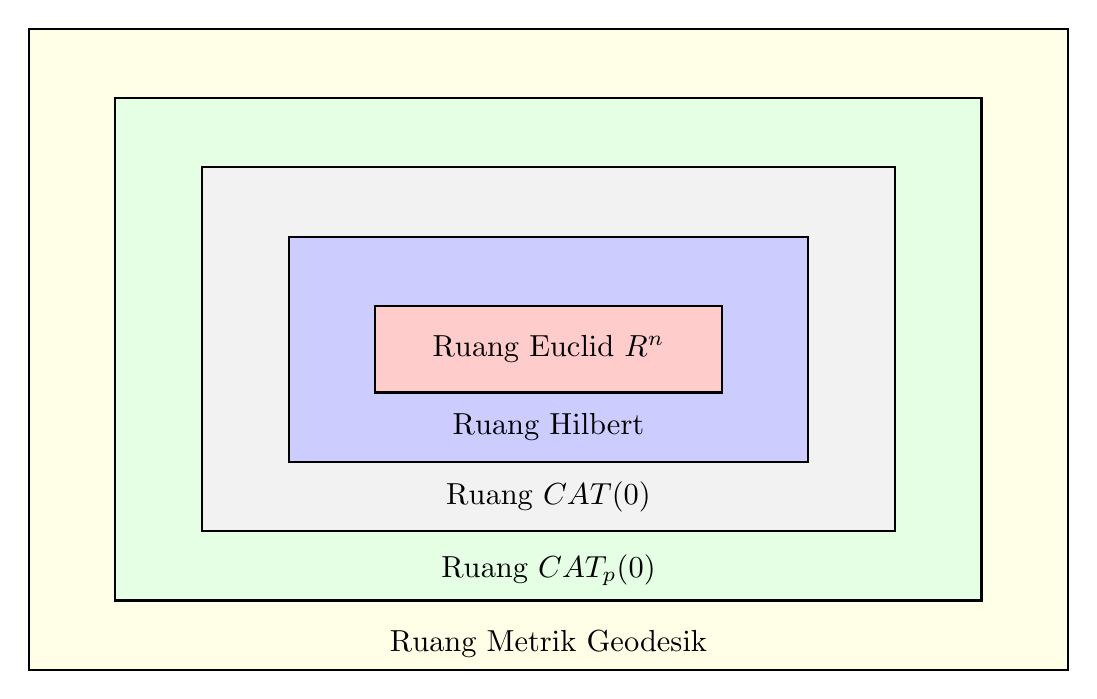
\begin{tikzpicture}[scale=1.1, every node/.style={transform shape}]


\draw[thick,fill=yellow!10] (-6,-3.7) rectangle (6,3.7);
\node at (0,-3.4) {Ruang Metrik Geodesik};

\draw[thick,fill=green!10] (-5,-2.9) rectangle (5,2.9);
\node at (0,-2.55) {Ruang $CAT_p(0)$};

\draw[thick, fill=gray!10] (-4,-2.1) rectangle (4,2.1);
\node at (0,-1.7) {Ruang $CAT(0)$};

\draw[thick, fill=blue!20] (-3,-1.3) rectangle (3,1.3);
\node at (0,-0.9) {Ruang Hilbert};

\draw[thick,fill=red!20] (-2,-0.5) rectangle (2,0.5);
\node at (0,0) {Ruang Euclid $\mathbb{R}^n$};


\end{tikzpicture}
\caption{\centering Hubungan ruang Euclid, Hilbert, $CAT(0)$, $CAT_p(0)$, dan ruang metrik geodesik}
\end{figure}


Pada bagian ini, dilakukan simulasi rekonstruksi citra tomografi berbasis skema iterasi Sabri. Transformasi maju $A$ yang digunakan adalah transformasi Radon, sedangkan himpunan batas $C$ dan $Q$ adalah himpunan bagian yang konveks dari suatu ruang Euclid, yang masing-masing merepresentasikan solusi \textit{feasible} untuk citra dan domain proyeksi. Pada simulasi ini, digunakan bahasa pemrograman Python dengan bantuan pustaka Scikit-image. Data citra yang digunakan adalah Shepp-Logan Phantom $x^*\in \mathbb{R}^n$ dengan resolusi $512\times 512$. Shepp-Logan Phantom dipilih karena merupakan model sintetik yang dirancang untuk menyerupai potongan gambar bagian dalam kepala manusia, sehingga sering digunakan dalam penelitian tomografi untuk menguji kemampuan algoritma rekonstruksi dalam membedakan struktur dengan tingkat kontras yang berbeda. Selanjutnya, data sinogram dibentuk sebagai $Q=Ax^*$ dengan menerapkan transformasi Radon pada sudut-sudut proyeksi yang terdistribusi merata pada interval $[0,180^{\circ})$. Tujuan simulasi ini adalah merekonstruksi citra $x^*$ berdasarkan data sinogram tersebut menggunakan skema iterasi Sabri. Untuk itu, digunakan pemetaan 
\begin{align}\label{eq:rekonoperator}
    T(x)=P_C(x-\gamma A^*(Ax-Q)),
\end{align}
dengan $A^*$ merupakan aproksimasi dari transformasi adjoin $A$ yang diperoleh menggunakan proyeksi mundur tanpa filter, serta $P_C$ menyatakan operator proyeksi ke himpunan batas $C=[0,1]^n$. 

Berikut ini diberikan diagram alir dari skema iterasi Sabri yang digunakan dalam simulasi rekonstruksi citra tomografi.
\begin{figure}[H]
    \centering
    \tikzstyle{startstop} = [ellipse, 
minimum width=5.5cm, 
minimum height=0.5cm,
text centered, 
draw=black]

\tikzstyle{io} = [trapezium, 
trapezium stretches=true, % A later addition
trapezium left angle=70, 
trapezium right angle=110, 
minimum width=6cm, 
minimum height=0.5cm, text centered, 
draw=black]

\tikzstyle{process} = [rectangle, 
minimum height=0.5cm, 
text centered, 
text width=8.5cm, 
draw=black]

\tikzstyle{decision} = [diamond, 
minimum width=2cm, 
minimum height=0.5cm, 
text centered, 
aspect=1.8,
inner sep=2pt,
draw=black]
\tikzstyle{arrow} = [thick,->,>=stealth]

\begin{tikzpicture}[node distance=1.4cm,scale=1, every node/.style={transform shape}]

% ===== Nodes =====
\node (start) [startstop] 
{Mulai};

\node (input) [io, below of=start,align=center,yshift=-0.3cm] 
    {Inisialisasi data Sinogram $Q$, gambar awal $x_0\in \mathbb{R}^n$,\\
     $k=0$, batas iterasi $K$, dan parameter $\gamma$, $\{a_k\},\{c_k\}\subseteq (0,1)$};

\node (hitung) [process, below of=input,yshift=-0.3cm] 
{Definisikan $T(x)$ sesuai persamaan \eqref{eq:rekonoperator}};

\node (qn) [process, below of=hitung] 
{$q_k = T\big((1-c_k)x_k + c_k T x_k\big)$};

\node (yn) [process, below of=qn] 
{$y_k = T(Tq_k)$};

\node (xn) [process, below of=yn] 
{$x_{k+1} = T\big((1-a_k)Tq_k + a_k Ty_k\big)$};

\node (decision) [decision, below of=xn, yshift=-0.8cm,align=center] 
{Apakah\\$k\geq K$?};

\node (stop) [startstop, below of=decision, yshift=-0.8cm] 
{Selesai};

% ===== Arrows =====
\draw [arrow] (start) -- (input);
\draw [arrow] (input) -- (hitung);
\draw [arrow] (hitung) -- (qn);
\draw [arrow] (qn) -- (yn);
\draw [arrow] (yn) -- (xn);
\draw [arrow] (xn) -- (decision);
\draw [arrow] (decision) -- node[anchor=east]{Ya} (stop);

\draw [arrow] (decision.east) -- ++(4,0) 
node[anchor=west]{Tidak}
|- (qn.east);

\end{tikzpicture}

    \caption{\centering Diagram alir skema iterasi Sabri untuk rekonstruksi citra tomografi}
    \label{fig:flowrekonstruksi}
\end{figure}

Selanjutnya, pada \ref{tab:parametersim} diberikan parameter-parameter yang digunakan dalam simulasi rekonstruksi citra tomografi tersebut.
\begin{table}[H]
    \centering
    \caption{Parameter simulasi rekonstruksi citra}
    \begin{tabular}{ll}
    \hline
    \textbf{Parameter} & \textbf{Nilai/Deskripsi}\\
    \hline
    Ukuran gambar     &  $512\times 512$ \\
    Sudut proyeksi     &  180 terdistribusi merata pada $[0^\circ, 180^\circ)$\\
    Transformasi maju $A$ & Transformasi Radon\\
    Transformasi adjoin $A^*$ & Proyeksi mundur tanpa filter\\
    Himpunan batas $C$ & $[0,1]^n$\\
    Nilai awal $x_0$ & $x_0=\mathbf{0}$\\
    Jumlah iterasi & 60\\
    Parameter $\gamma$ & Konstan: 0.00245\\
    Parameter $a_n,c_n$ & Konstan: $a_n=0.42, c_n=0.31$\\
    Implementasi & Google Colab dengan scikit-image, matplotlib\\
    \hline
    \end{tabular}
    \label{tab:parametersim}
\end{table}





Data awal dari simulasi tersebut disajikan pada \ref{fig:rekoncit}. Kemudian hasil simulasi dari rekonstruksi citra tersebut pada iterasi ke-5, 10, 30, dan 60 diberikan oleh \ref{fig:rekoncit2}. Pada iterasi ke-5, terlihat bahwa derau dari citra tersebut masih cukup tinggi, yang juga tertera pada nilai (\textit{peak signal noise ratio}) PSNR, yaitu 22.03 dB. Nilai PSNR dari citra tersebut juga makin membesar pada iterasi ke-10 dan 30, serta untuk iterasi ke-60, nilai PSNR citra tersebut adalah 35.61 dB, yang mengindikasikan semakin sedikit derau pada citra.  
\begin{figure}[H]
    \centering
    \includegraphics[width=\linewidth]{Bab_4/citrafix.png}
    \caption{Data awal sinogram dan citra asli}
    \label{fig:rekoncit}
\end{figure}
\begin{figure}[H]
    \centering
    \includegraphics[width=\linewidth]{Bab_4/citrafix2.png}
    \caption{Hasil rekonstruksi citra pada iterasi ke-5, 10, 30, dan 60}
    \label{fig:rekoncit2}
\end{figure}
Pada \ref{tab:msepsnr}, diberikan nilai metrik PSNR dan MSE dari citra hasil rekonstruksi pada tiap iterasinya. Terlihat bahwa nilai galat, yaitu (\textit{mean squared error}) dari citra tersebut relatif kecil pada iterasi ke-60, yaitu $2.7\times 10^{-4}$, dibandingkan dengan galat pada iterasi pertama, yaitu $2\times 10^{-2}$. Terlihat pula bahwa nilai metrik PSNR dan MSE tersebut turun pada tiap iterasinya, sesuai dengan peningkatan kualitas citra pada \ref{fig:rekoncit2}, yang menunjukkan bahwa skema iterasi Sabri dapat digunakan dalam rekonstruksi citra tomografi.
\begin{longtable}{|c|>{\centering\arraybackslash}p{4cm} | >{\centering\arraybackslash}p{4cm} |}
\caption{\centering MSE dan PSNR Rekonstruksi Citra}\label{tab:msepsnr}\\
\hline
{\textbf{Iterasi ke-$n$}} & {\textbf{MSE}} & {\textbf{PSNR}} \\
\hline
\endfirsthead 
\multicolumn{3}{c}{\centering \thetable{} -- Lanjutan dari halaman sebelumnya} \\
\hline
{\textbf{Iterasi ke-$n$}} & {\textbf{MSE}} & {\textbf{PSNR}} \\
\hline
\endhead 
% \multicolumn{3}{c}{{Lanjut pada halaman berikutnya}} \\
\hline
\endfoot 
\hline
\endlastfoot
\hline
1  & 0.020302 & 16.924673 \\
2  & 0.013587 & 18.668847 \\
3  & 0.010072 & 19.968693 \\
4  & 0.007823 & 21.066098 \\
5  & 0.006272 & 22.026258 \\
6  & 0.005149 & 22.882519 \\
7  & 0.004309 & 23.655780 \\
8  & 0.003664 & 24.360387 \\
9  & 0.003157 & 25.006683 \\
10 & 0.002753 & 25.602432 \\
11 & 0.002425 & 26.153733 \\
12 & 0.002155 & 26.665575 \\
13 & 0.001931 & 27.142128 \\
14 & 0.001743 & 27.587012 \\
15 & 0.001584 & 28.003332 \\
16 & 0.001448 & 28.393736 \\
17 & 0.001330 & 28.760530 \\
18 & 0.001229 & 29.105746 \\
19 & 0.001140 & 29.431187 \\
20 & 0.001062 & 29.738458 \\
21 & 0.000993 & 30.028997 \\
22 & 0.000932 & 30.304104 \\
23 & 0.000878 & 30.564968 \\
24 & 0.000829 & 30.812682 \\
25 & 0.000786 & 31.048254 \\
26 & 0.000746 & 31.272582 \\
27 & 0.000710 & 31.486496 \\
28 & 0.000678 & 31.690770 \\
29 & 0.000648 & 31.886142 \\
30 & 0.000620 & 32.073295 \\
31 & 0.000595 & 32.252847 \\
32 & 0.000572 & 32.425370 \\
33 & 0.000551 & 32.591386 \\
34 & 0.000531 & 32.751347 \\
35 & 0.000512 & 32.905658 \\
36 & 0.000495 & 33.054684 \\
37 & 0.000479 & 33.198752 \\
38 & 0.000464 & 33.338168 \\
39 & 0.000449 & 33.473223 \\
40 & 0.000436 & 33.604183 \\
41 & 0.000424 & 33.731285 \\
42 & 0.000412 & 33.854741 \\
43 & 0.000400 & 33.974740 \\
44 & 0.000390 & 34.091450 \\
45 & 0.000380 & 34.205025 \\
46 & 0.000370 & 34.315610 \\
47 & 0.000361 & 34.423339 \\
48 & 0.000353 & 34.528338 \\
49 & 0.000344 & 34.630725 \\
50 & 0.000336 & 34.730611 \\
51 & 0.000329 & 34.828102 \\
52 & 0.000322 & 34.923289 \\
53 & 0.000315 & 35.016256 \\
54 & 0.000309 & 35.107081 \\
55 & 0.000302 & 35.195841 \\
56 & 0.000296 & 35.282605 \\
57 & 0.000291 & 35.367439 \\
58 & 0.000285 & 35.450403 \\
59 & 0.000280 & 35.531556 \\
60 & 0.000275 & 35.610951 \\
\hline
\end{longtable}
